\documentclass[draft]{figs/agu/agujournal2025}
\usepackage{amsmath}
\usepackage{booktabs}
\usepackage{float}
\usepackage{tikz}
\usepackage{mathrsfs}
\usepackage{soul}
\usepackage{amssymb}
\usepackage{colortbl}
\usetikzlibrary{matrix, shapes, positioning, arrows.meta, fit, backgrounds, calc}

\AtBeginDocument{%
  \setlength{\RaggedRightRightskip}{0pt plus 2em}%
  \RaggedRight
  \setlength{\emergencystretch}{2em}%
  \raggedbottom%
}

\begin{document}

\journalname{Space Weather}

\title{A Comparative Analysis of High Energy Proton Flux Measured at Lagrange Point 1 Forecasting Hetero Models  with Time Series Transformers}

\authors{Lewis Adkins\affil{1}}
\affiliation{1}{Space Weather Lab Group, George Mason University}

\authoraddr{Lewis Adkins, Space Weather Lab Group, George Mason University, email: ladkins8@gmu.edu}
\authorrunninghead{Adkins}
\titlerunninghead{Comparative Analysis of Proton Flux Forecasting}

\keypoints
{Persistence nowcasts can be as reliable as more advanced forecasting models when predicting solar energetic particles.}
{Bootstrap analysis can be an effective method to measure the prediction variability of models.}
{Positional encoding methods in transformers offer little to no improvement in forecasting tasks.}

\maketitle
\clearpage
\section{Abstract}
\label{sec:abstract}
Solar energetic particles are a crucial limb in the solar storm anatomy.  Space and Earth-based infrastructure are at risk 
due to damage caused by the bombardment of the particles in space and in the upper ionosphere. Satellite, avionic, and communication systems can degrade or completely malfunction  if the particle intensity is too high.
Previous physics and statistical models have made progress in forecasting SEP events, however the reliance on other correlated solar storm parameters and the computational cost
inhibits the ability to make real time warnings. Machine learning models has shown improvements in generalizing SEP behavior but issues with long range dependencies
and lack of parallelization has led to the time series transformers as a viable alternative. We construct three time series transformers with different positional encoding methods to 
train on past high energy proton and relativistic electron fluxes  of 5 minute cadence to predict 30 minutes to 1 hour ahead. We replicate a neural network and recurrent neural network designed for SEP 
forecasting to compare the performance. Included also is a multivariate linear regression model, a forecasting matrix model, and a persistence model. A bootstrap analysis of the time series is performed to measure the forecast behavior of the models. Our results indicate that
a persistence model outperforms on almost all key metrics with less variability in results. Machine learning models were able to reduce the time lag between proton predictions. 



\section{Plain English Summary}
\label{sec:plain_english_summary}
Solar Energetic Particles (SEPs) can be very dangerous to space and Earth-based infrastructure. Because electrons are able to travel to Earth much faster than protons, they can act as a precursor to incoming SEP events. 
Previous models incorporate other aspects of solar storms that correlate with these SEP events. Using statistical and empirical methods, they are able to predict incoming proton storms to some degree of accuracy. 
Machine learning showed improvements to the predictions and to attempt to outperform, we use a variety of transformer models that can predict proton flux on the same particle dataset 30 minutes and 1 hour out. Our 
results show that previous notions of machine learning improvements and transformers show little improvements to very rudimentary models such as persistence.
\clearpage
\section{Introduction}
The space weather environment is home to many hazards that put humans and their artificial satellites at risk \cite{eastwood2017economic}. 
Solar Energetic Particles (SEPs) are bursts of high energy protons $>10$ MeV, electrons and $\alpha$ particles following the magnetic field lines from the Sun reaching relativistic speeds $(\approx 0.9c)$. Coronal Mass Ejections (CMEs) drive shock waves that accelerate SEPs to tens of GeV and flux $\geq 10$ MeV making them difficult to shield \cite{reames2021solar}.
SEPs are one of many species in the extra-terrestrial ecosystem; however, protons $>10$ MeV are one of the greatest offenders damaging electronic components on satellites, aircraft, high frequency communications, and human health, making reliable forecasting essential \cite{eastwood2017economic}.
SEP relativistic  electrons ($0.95c$, $1$ MeV) are always present during storm events and precede slower incoming SEP ($0.25c$, $30$ MeV) protons due to less scattering  \cite{nunez2018hesperia}.
This simple relationship has been the basis of a portion of forecast models predicting high energy protons at $10$ pfu.

Physics models that simulate heliospheric transport and particle acceleration processes are computationally expensive and are usually studied to understand underlying processes rather than generating predictions \cite{Camporeale2019,kasapis2026review}.
The issue with all physics-based SEP models is that they may have poorly constrained free parameters such as diffusion coefficients and which specific magnetic field line to select to produce a prediction for the particle spectrum at the observer's location \cite{whitman2023}.
Empirical and statistical models provide predictions but rely heavily on historical correlations leaving probabilities of an event to occur \cite{whitman2023}. Together, physics, statistical, and empirical models are limited by uncertain inputs and must trade off realistic behavior with forecast timeliness \cite{yu2026}.

Machine Learning (ML) models have had major breakthroughs in the application of space weather due to the large availability of in situ observations and recent advancements in Graphics Processing Unit (GPU) computing \cite{Camporeale2019}. ML models predicting SEPs with space weather properties demonstrated improved results establishing reliable forecast methods \cite{Posner2024,yu2026,nunez2022umasep,Dayeh2024}.
With the recent development of self-attention architectures, transformers, \cite{vaswani2017attention}, there is still room for improvements. Recurrent models struggle with long-range dependencies, convolution models require deep stacking to enlarge receptive fields, and both scale suboptimally to high-dimensional and high-volume data \cite{zhao2026transformersurvey}. Transformers evaluate the totality of input data in parallel to generate reliable, accurate outputs. Their architecture allows for optimal scaling \cite{vaswani2017attention}. Because the introduction of transformers is recent, there are limited applications in predicting space weather, therefore a fully realized comparative analysis of forecasting performance is necessary and would provide much insight for other modelers.

We analyze   time series  SEP data (5-minute cadence) recorded by the Solar and Heliospheric Observatory Comprehensive Suprathermal and Energetic Particle Analyzer--Electron Proton Helium Instrument
(SOHO-COSTEP-EPHIN) located at Lagrange Point 1 (L1). We compare transformer models to a collection of SEP forecasting models of all types under a battery of assessments. These include multilayer perceptron neural network (NN) and recurrent neural network (RNN) models \cite{torres2025machine}, a physics model using an electron increase parameter matrix \cite{posner2007forecasting}, and simple statistical and empirical models, persistence and linear regression.  
Our tests include a fixed 2-hour time window of particle fluxes as an input to predict a single proton flux value at either $30$ minutes or $60$ minutes ahead. Additionally, 
expanding the input time window, increasing forecasting time, and parameter sizes of our models will give us a holistic diagnosis of the performances
between the models.

Across  all forecasting models types, each model reads in solar storm parameters, measures resulting metrics, and performs analysis that is different than the next. No two model studies
analysis is the same. Some studies do not include a naive persistence model to compare against. This study also hopes to establish standards of metric acquisition and scoring
to properly compare forecasting models to each other similar to the time series transformer field. 

Section \ref{sec:relatedwork} will discuss related work on transformer applications.
Section \ref{sec:approach}  will report which transformer models we developed and why,  and reintroduce previously mentioned models more in depth. A summary of selected metrics will be provided to compare forecasting accuracy. Finally, we provide an outline of our battery assessment in detail.
Section \ref{sec:experimentalevaluation} will show our evaluation of the model performances for each test with analysis.
Section \ref{sec:conclusion} will summarize and discuss future work, potential improvements and limitations.

\clearpage
\section{Related Work}
\label{sec:relatedwork}

\textbf{SEP ML Forecasting}
Machine learning has been applied to SEP forecasting mainly as an event-occurrence problem, using solar-source precursors.
\citeA{boubrahimi2017prediction} used other satellites  like GOES and their proton and X-ray fluxes data as multivariate time series for a  interpretable decision trees to predict $>100$ MeV SEP events
\citeA{engell2017sprints} developed SPRINTS, which also uses GOES X-ray flare metadata using statistical, and machine-learned decision tree models.
\citeA{laurenza2018esperta} adapted the ESPERTA empirical model, using flare location, soft X-ray fluence, and 1 MHz radio fluence, providing short-term warnings of moderate-to-extreme solar proton events.
\citeA{aminalragia2021sep} trained neural networks on GOES soft X-ray measurements of solar flares to predict whether a flare would be followed by an SEP event.
\citeA{lavasa2021predictability} treated SEP prediction as a is happening/ is not happening result and compared several machine learning methods on flare and coronal mass ejection data. CME speed,
CME width, and flare soft X-ray fluence were concluded to be informative features. \citeA{kasapis2022interpretable} used support vector machines and regression models on active region magnetograms from SOHO/MDI
to forecast SEP events during Solar Cycle 23. These studies predict whether an event will occur from solar-source precursors, using decision trees, support vector machines,
ensembles, and feedforward neural networks. In contrast, this study forecasts the time profile of the >10 MeV proton flux from relativistic electrons measured in situ at L1
\cite{posner2007forecasting,torres2025machine},
and evaluates attention-based transformer architectures, which have not been applied to this task.

\textbf{Time Series Transformer Applications}
Since their introduction for machine translation \cite{vaswani2017attention}, transformers have been adapted to time series forecasting across many fields \cite{zhao2026transformersurvey}.
Time Series Transformer uses learnable positional encodings with unsupervised pre-training to perform well when data are scarce \cite{zerveas2020transformer}.
More recent models such as Chronos treat forecasting as a language-modeling task and pre-train on many datasets to forecast without task-specific training \cite{ansari2024chronos}.
These architectures have been applied to stock market prediction, clinical and physiological monitoring, battery state-of-health estimation,
and traffic flow forecasting \cite{cai2020traffictransformer,zhao2026transformersurvey}, but rarely to space weather.
Their advantage is not guaranteed, however. Simple baselines can match or beat them: a naive forecast that
repeats the last observed value outperformed transformer models on exchange-rate data \cite{zeng2022transformers},
and transformers tend to overfit when training data are limited \cite{zhao2026transformersurvey}.
\citeA{zhao2026transformersurvey} further note that their performance depends strongly on the choice of positional encoding.
\clearpage
\section{Approach}
\label{sec:approach}
SEP events are comprised of high energy particles such as protons, electrons and alpha particles, with protons being the highest risk to space and ground based infrastructure \cite{wilkinson1991tdrs}.
At 1 AU, relativistic electrons experience less scattering than protons when traveling to earth. Because of this, an early wanring forecast model can be created that only uses preceding
relativistc electrons to warn us of high energy protons \cite{posner2007forecasting}, \cite{torres2025machine}.  A time series of raw particle channels from COSTEP is used for forecasting using time series transformers.
We build a series of transformer models with different encoding architectures that captures the correlation of proton and electron intensity
using multiple methods.

In Section \ref{sec:input} we discuss the particle time series and the instrument. Section \ref{sec:transformer} provides an explantion of what transformers are and they differ
to previous machine learning models. \ref{sec:positionalencodingmethods} justifies the chosen positional encodings architectures.

\subsection{Input}
\label{sec:input}

\begin{figure}[!htbp]
    \centering
    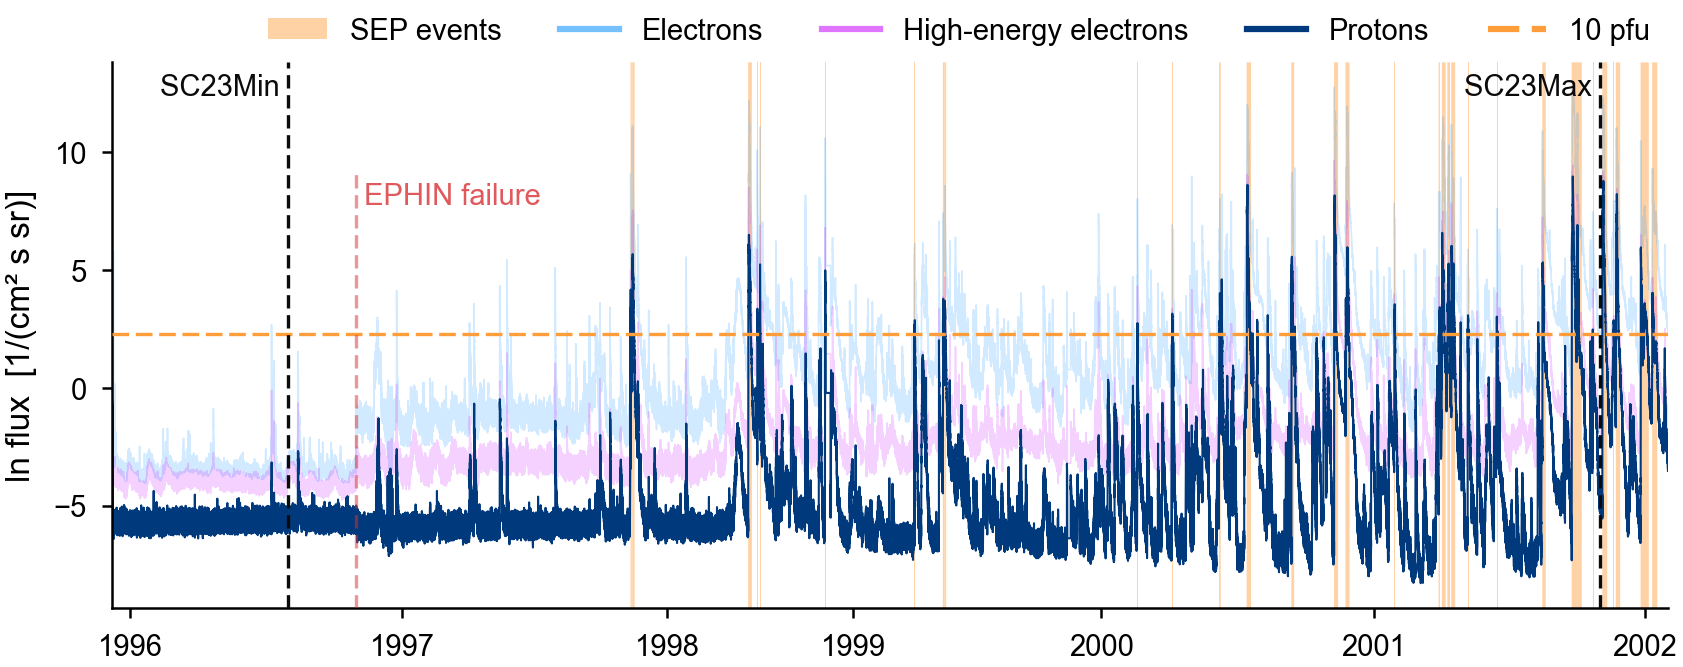
\includegraphics[width=\textwidth]{figs/approach/input/flux_series.png}
    \caption{SOHO COSTEP-EPHIN dataset from 1995-2002}
    \label{fig:data_overview_single}
\end{figure}

The particle channel data are obtained from the Comprehensive Suprathermal and Energetic Particle Analyzer - Electron Proton Helium Instrument (COSTEP-EPHIN)  on the Solar and Heliospheric Observatory (SOHO). SOHO first launched on December 2nd 1995 to take in situ of energy depostion and particle acceleration in the solar atmosphere \cite{SOHOCOSTEPEPHINCDFPT1M}.
SOHO orbits between the earth and sun around Lagrange Point 1 (L1), which is approximately 1.5 million kilometers from earth. L1 is an ideal location 
for space weather isntrumetns as any satelltie situatued there enjoys an uninteruppted view of the sun.
The EPHIN instirments switched to failure mode that reduced the energy ranges it was able to read on October of 1996 \cite{kuhl2019revising}.
\cite{torres2025machine} provides a dataset of 39 SEP identified events using the particle data recorded by COSTEP-EPHIN. Two relatavistic electron intensities channels $\geq$0.25 and $\geq$0.67 MeV \cite{mullermellin1995costep} are the precursors for our incoming protons. Proton channels are seperated into four energy channels (P4,P8,P25, P41) each corresponding to  different energy ranges.
Proton channel P4 corresponds to the energy range $4.3 - 7.8 \text{ MeV}$, P8 corresponds with $7.8-25 - 7.8 \text{ MeV}$,  P25 corresponds with  $25 - 40.9 \text{ MeV}$, and P41 corresponds with $40.9 - 53 - 7.8 \text{ MeV}$. To retreive a $>10$ MeV proton flux channel, a sum of the energy integrated fluxes P8,P25, and P41 channels minus the range
$7.8-10$ MeV is performed. The latter channel is determined by the a power law spectrum  interpolation of the first two channels, P4 and P8, differential fluxes and their mean energies \cite{torres2025machine}.

SEP events were then identified for storms larger than 10 proton flux unit (pfu). Each event is partitioned into phases to highlight definable features: Onset, Threhsold, Peak, End.
The onset is defined when the flux rises three times the error bar above the pre-event background, the threshold is when the flux first crosses over 10 pfu and the end time is when it drops again below 2 pfu.\cite{torres2025machine}.

\subsection{Why Transformers}
the computaitonal power of a transfomrer can be parelized requireing less operaitons. Long range dependencies can be handled much easier
with larger winow lengths. Inputs  passes forward and back signals that help to make predictions.
As the input window length grows, the harder it is to learn long range dpeendencies on RNN and NN modles \cite{zhao2026transformersurvey}. Self Attention could yield more interpretabhle models \cite{vaswani2017attention}.
NN and RNN scale suboptimally to large datasets compared to transformer models \cite{zhao2026transformersurvey}

Physics based models simulating particle accelration and trnasport processes are omputionatially expensive and with the limited amount of data limited \cite{Camporeale2019} \cite{yu2026} \cite{kasapis2026review}.
Fruthermore lmiations in forecast timeliness forces a trade off with realism \cite{yu2026}.

\subsection{Transformers}
\label{sec:transformer}

The original transformer is comprised of encoder-decoder stacks with built in self attention modules that translates inputs $\mathbf{X}$ into vectors $\mathbf{Z}$,
identifies correlations and relationships, and outputs a sequence of predictions $\mathbf{Y}$. The encoder stack handles the $\mathbf{X \rightarrow Z}$ transformations while the decoder  handles $\mathbf{Z \rightarrow Y}$ \cite{vaswani2017attention}.
Because we are only predicting a singular timestamp of proton flux in the future, we drop our decoder stacks as its purpose is to gneerate a sequence of 
outputs from $\mathbf{Y}$ rather than one value \cite{vaswani2017attention}.

For our time series data, we use two hours of historical particle flux data of our two electron channels and $>10$ MeV proton channel. The magnitude in differences of fluxes between our channels  is large enough to cause 
unstable trianing and testing therefore we apply a natural $\log$ transformation to the entire dataset, resulting compressing the mean and  variance on the same scale. The standard method is to 
subtract by the mean and divide by the standard deviation, a process called "standardization". To ensure our NN and RNN
align with \cite{torres2025machine} model results, the prior method is selected instead to replicate \cite{torres2025machine}

We set $t$ to indicate present time. Becasue of the cadence of 5 minutes,
 $t - 25$ timestamps creates twenty-four 5-min intervals of particle flux forming a window of inputs before and including the current time. For each window, we define an input sample:
$$
\mathbf{X} \in \mathbb{R}^{l \times v} = \mathbb{R}^{25 \times 3}
$$
where $l$ is the length of the input window and $v$ is the number of variates. A processes that translates our particle fluxes at each timestep into transformer
readable vecotrs, embedding, is calculated by:
$$
\mathbf{
U} = \mathbf{XW_p}^T + \mathbf{1b_p}^T, \mathbf{1} \in \mathbb{R}^{l \times 1}
$$
$\mathbf{W_p} \in \mathbb{R}^{d \times v}$ and $\mathbf{b_p} \in \mathbb{R}^{d}$ are weighted and bias vectors respectively. They are initialized randomly at the start of training and then used to compute $\mathbf{U} \in \mathbb{R}^{l \times d}$.
After every training cycle, these vectors  updates and learn to optimize minimizing loss, error.
$d$  is the dimension of the embedding vector that represents our inputs. For large $d$, inputs are characterized at a higher resoltution allowing  models to learn finer grain patterns at the cost of compuational power and risk of overfitting. 
The number of parameters in a model is proportional to the size of $\mathbf{W_p}$ and $\mathbf{b_p}$ \cite{vaswani2017attention} \cite{zerveas2020transformer}

\begin{table}[!htbp]
\centering
\caption{Total number of trainable parameters for each model.}
\label{tab:param-count}
\begin{tabular}{l r}
\toprule
Model & Parameters \\
\midrule
NN          & 2,311 \\
RNN         & 3,181 \\
\midrule
Sinusoidal  & 3,361 \\
Zero-Init   & 3,761 \\
RoPE        & 3,361 \\
\bottomrule
\end{tabular}
\end{table}


To match parameter size of \cite{torres2025machine} we use $d = 16$. Our transformer models are slighlty larger than the RNN and NN provided by \cite{torres2025machine}. A model size $d=8$ would 
greatly reduce the models far below the parameter count of RNN and NN.  Table \ref{tab:param-count} provides
a count of all parameters in each machin learning model in this study.
The RNN and NN are implemented  with two layers: One layer is hidden with 30 units and then a second dense single output layer.
The RNN is comprised of  Gated Recurrent Units (GRU) for its  hidden layers while the NN uses hidden layers.
The NN model uses the same three channels for 25 timestep intervals.
The RNN  has the 30 GRU units plus our three channel input \cite{torres2025machine}. 
All models (RNN,NN, transformers) minimize the loss function with mean square error during training.
\begin{figure}[H]
    \centering
    \resizebox{0.6\textwidth}{!}{
    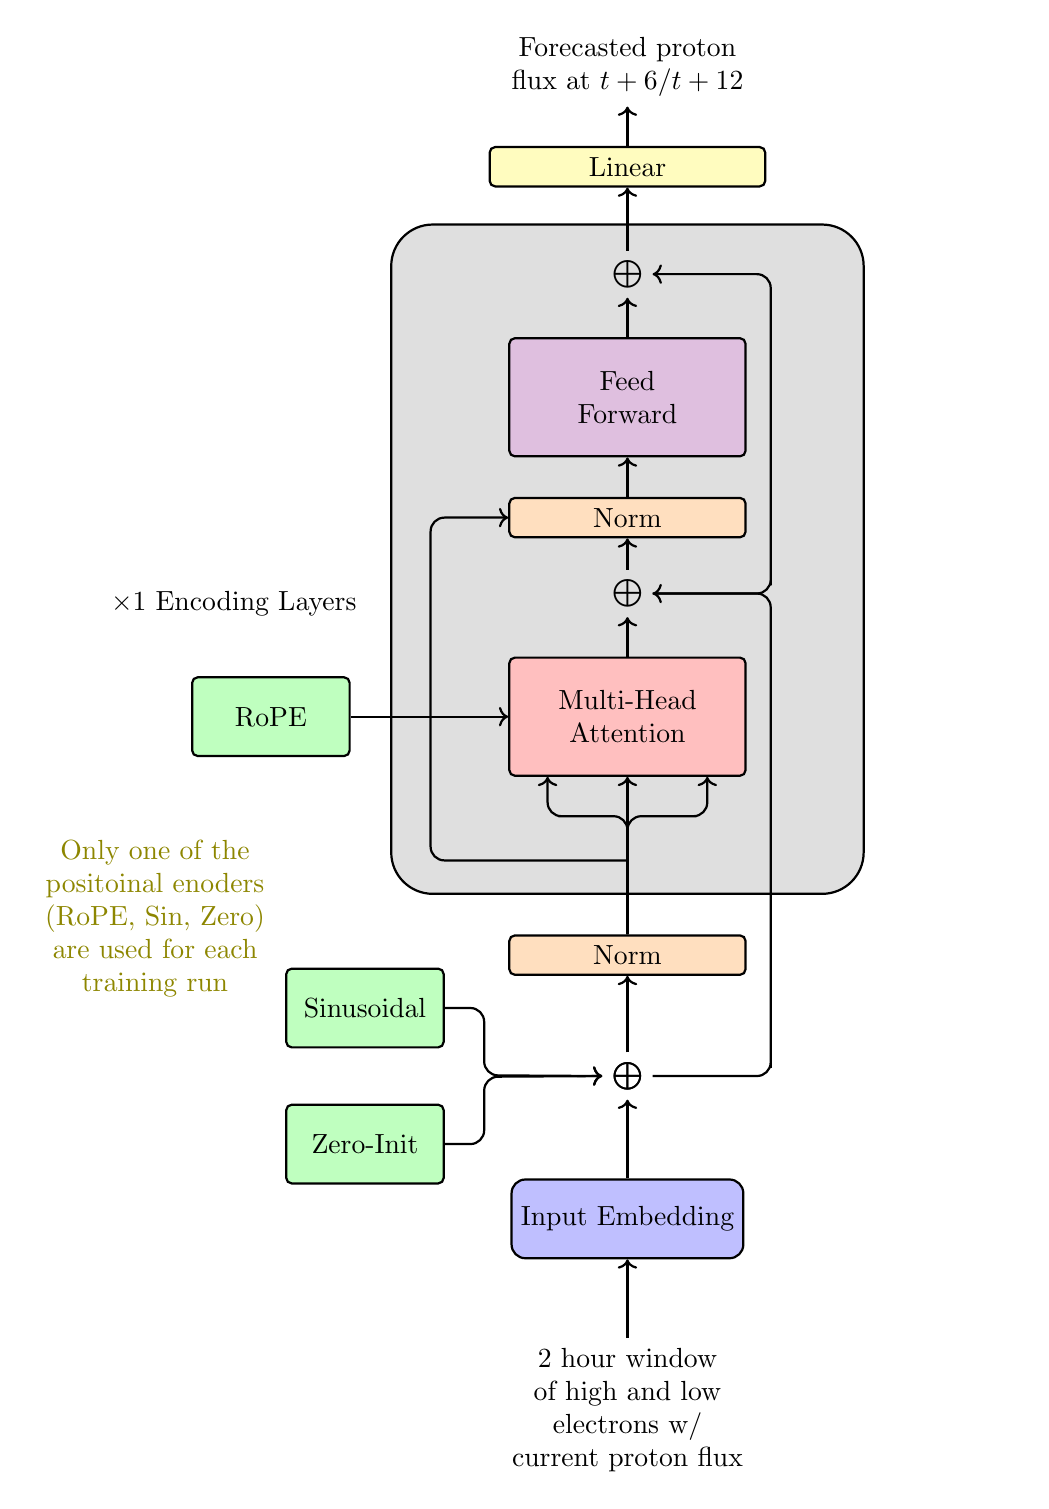
\begin{tikzpicture}[
        pebox/.style={
            draw, rounded corners=2pt, fill=green!25,
            minimum width=2cm, minimum height=1cm, thick,
        },
        mhbox/.style={
            draw, rounded corners=2pt, fill=red!25,
            minimum width=3cm, minimum height=1.5cm, thick,
        },
        normbox/.style={
            draw, rounded corners=2pt, fill=orange!25,
            minimum width=3.0cm, minimum height=.5cm, thick,
        },
        feedforwardbox/.style={
            draw, rounded corners=2pt, fill=violet!25,
            minimum width=3.0cm, minimum height=1.5cm, thick,
        },
        linearbox/.style={
            draw, rounded corners=2pt, fill=yellow!25,
            minimum width=3.5cm, minimum height=.5cm, thick,
        },
        softmaxbox/.style={
            draw, rounded corners=2pt, fill=teal!25,
            minimum width=3.5cm, minimum height=.5cm, thick,
        },
        scale = 1
    ]

        % outer container: the whole encoder block


        \node (pe) at (0,-8) {$\bigoplus$};
        \node[
            draw,
            rounded corners=15pt,
            fill=gray!25,
            minimum width=6cm,
            minimum height=8.5cm,
            thick,
            above = 20mm of pe,
        ] (outer){};

        % positional-encoding options, stacked left of pe: RoPE level with pe,
        % Sinusoidal/Zero-Init symmetric above/below it -- no manual coordinates
        
        \node[text= olive, text width = 3 cm, align=center](pe_disclaimer) at (-6,-6){Only one of the positoinal enoders (RoPE, Sin, Zero) are used for each training run };
        \node[pebox, above left =.5mm and 2cm of pe] (Sinusoidal) {Sinusoidal};
        \node[pebox, below left =.5mm and 2cm of pe] (Zero-Init) {Zero-Init};
        \node[mhbox, above=35mm of pe, text width = 2 cm, align=center] (MultiHead) {Multi-Head Attention};
        \node[normbox, above = 1.5 cm of MultiHead] (norm1){Norm};
        \node[pebox, left=2cm of MultiHead] (RoPE) {RoPE};
        \node[
            draw, rounded corners=5pt, fill=blue!25,
            minimum width=2cm, minimum height=1cm, thick,
            below=10mm of pe,
        ] (Input_Embedding) {Input Embedding};
        \node[feedforwardbox, above =  5mm of norm1, text width = 2 cm, align=center](FeedForward){Feed Forward};
        \node[below= 1cm of Input_Embedding, text width = 3cm, align=center](input) {2 hour window of high and low electrons w/ current proton flux};
        \node[normbox, below = 2cm of MultiHead](norm2){Norm};


        \node[align = center] at (-5,-2){$\times 1$ Encoding Layers};
        \node[above = 5mm of MultiHead] (pe2) {$\bigoplus$};
        \node[above = 5mm of FeedForward] (pe3) {$\bigoplus$};
        \node (pe) at (0,-8) {$\bigoplus$};
        \node[linearbox, above = 8mm of pe3](linear){Linear};

        \draw[->,thick](input.north) -- (Input_Embedding.south);
        \draw[->, thick, rounded corners=5pt] (Input_Embedding.north) -- (pe.south);
        \draw[->, thick, rounded corners=5pt] (RoPE.east) -- (MultiHead.west);
        \draw[->, thick, rounded corners=5pt] (Zero-Init.east) -| ++(5mm,8.55mm) -- (pe.west);
        \draw[->, thick, rounded corners=5pt] (Sinusoidal.east) -| ++(5mm,-8.55mm) -- (pe.west);
        \draw[->, thick, rounded corners=5pt] (pe.east) -| ++(15mm,0) |- (pe2.east);
        \draw[->, thick, rounded corners=5pt] (pe2.east) -| ++(15mm,0) |- (pe3.east);
        \draw[->, thick, rounded corners=5pt] (norm2.north) |- ++(-7mm,15mm) -| ($(MultiHead.south west) + (5mm,0)$);
        \draw[->, thick, rounded corners=5pt] (norm2.north) |- ++(7mm,15mm) -| ($(MultiHead.south east) - (5mm,0)$);
        \draw[->, thick] (norm2.north)  -- (MultiHead.south);
        \draw[->, thick] (pe.north)  -- (norm2.south);
        \draw[->,thick](norm1.north) -- (FeedForward.south);
        \draw[->,thick](FeedForward.north) -- (pe3.south);
        \draw[->, thick](pe3.north) -- (linear.south);
        \draw[->, thick , rounded corners=5pt]($(pe)!0.60!(MultiHead)$) -| ++(-25mm, 15mm) |- (norm1.west);
        \draw[->,thick](MultiHead.north)--(pe2.south);
        \draw[->, thick](pe2.north)--(norm1.south);
        \draw[->,thick, text width = 3 cm, align=center](linear.north) -- ++(0,5mm) node[above] {Forecasted proton flux at $t+6$/$t+12$};
        \path (5,-2); % invisible point, balances the bounding box against the "$\times 1$" label on the left
    \end{tikzpicture}
    }
    \caption{Generic transformer architecture where positional encoding methods are indicated to show the difference between all models}
    
    \label{fig:transformer-pe}
\end{figure}


\subsection{Positional Encoding Methods}
\label{sec:positionalencodingmethods}

Transformer models computes updates in $\mathbf{W_p}$ and $\mathbf{b_p}$ in parallel. This allows for large input sequences
to be read at the same time without "forgetting" related timestamps that are far apart from eachother in the window.  
Any reshuffling of the vectors that make  up $\mathbf{U}$ has no effect on the the update calculation. 
Additional positional information must be injected to bring  context to our input window \cite{vaswani2017attention}.
For all input vectors $\mathbf{u_w}$ we add a $\mathbf{w_{\text{pos}, w}}$:
$$
\mathbf{U' = U + W_{\text{pos}}} , \mathbf{W_\text{pos}} \in \mathbb{R}^{l \times d}
$$
RNNs and NNs in contrast, reads the inputs sequentially learning order inherently.

The particle flux dataset is small, therefore different positional encoding (PE) could effect predictions.
PE is said to be a major factor in "length generalization", ability to extrapolate effectively  large sequences of events
from smaller training context windows. Transformers without PE outperform those with explicit PE methods \cite{kazemnejad2023impact}. 


\subsubsection{Sinusoidal Positional Encoding}
\label{sec:sinusoidalPE}
Sinusoidal positional encoding was first introduced in the original proposed transformer architecture paper \cite{vaswani2017attention}.
It is an absolute position encoding method that uses sinusoidal and cosine functions of different frequencies to encode the positional indexes of tokens in a sequence.
The input window is split into smaller chunks called tokens. For each token, a vector of dimension, $d$ is generated. The vector is determined by the position, $pos$, in the window and the length of the vector, $d$.
$i$ is the dimension of the PE vector. Odd and even indexes in the vector are determined by \eqref{cosPE} and \eqref{sinPE} respectively. This gives us a new vector $\mathbf{w_\text{pos}} \in \mathbb{R}^{l \times 1}$.
\eqref{sinPE} and \eqref{cosPE} to represent a linear relationship between two encoded positions.

\begin{equation}
    \label{sinPE}
    PE_{(pos,2i)} = \sin (pos / 10000^{2i/d})
\end{equation}


\begin{equation}
    \label{cosPE}
    PE_{(pos,2i+1)} = \cos(pos/10000^{2i/d})
\end{equation}


 The frequency decreases exponentially by a scale factor as the position in the model dimensions increase.
 Similarly stated in Section \ref{sec:transformer}, in the short term we can map small patterns in data, a $\sin/\cos$ function with a high frequency.
 At large vector indexes the frequency greatly decreases, taking on a more linear relationship.
 The positions are encoded uniquely based on value and position, allowing it to scale to unlimited sequence lengths. \cite{vaswani2017attention}

\subsubsection{Rotary Positional Embedding}

Rotary Positional Embedding (RoPE) is a PE method that stores the poistion infomration of a token,$m$ in a squence
in the total rotation of that query-key vectors by some angle $\theta_i$. The rotation amount is calculated by:
$$
\theta_i = 10000^{-2(i-1)/d}, \left\{i \in \mathbb{Z} \Bigg| 1 \leq i \leq \frac{d}{2}\right\}
$$
The rotation matrix is then applied to the token:
$$
r_{\theta_i} =  
\begin{bmatrix} 
\cos (m\theta_i) & -\sin (m\theta_i)  \\
\sin (m\theta_i) & \cos (m\theta_i )
\end{bmatrix}
$$
To generalize we stack our rotation values $\Theta = [\theta_1, ..., \theta_{d/2}]$ form the rotary matrix:

\begin{equation}
\mathbf{R}^{d}_{\Theta,m} =
\begin{pmatrix}
r_{\theta_1} & \mathbf{0} & \cdots & \mathbf{0} \\
\mathbf{0} & r_{\theta_2} & \cdots & \mathbf{0} \\
\vdots & \vdots & \ddots & \vdots \\
\mathbf{0} & \mathbf{0} & \cdots & r_{\theta_{d/2}}
\end{pmatrix}
= \operatorname{diag}\!\left(r_{\theta_1}, r_{\theta_2}, \dots, r_{\theta_{d/2}}\right)
\end{equation}
where each $\mathbf{0}$ is a $2 \times 2$ block of zeros, so $\mathbf{R}^{d}_{\Theta,m} \in \mathbb{R}^{d \times d}$.

Unlike Section \ref{sec:sinusoidalPE} and Section \ref{sec:ZeroPE}, the transformations are applied
directly to the self attention block as illustrated in \ref{fig:transformer-pe}, see Section \ref{sec:self-attention}.
The attention weight between two query-key in a sequence, $\mathbf{q}_m^T \mathbf{k}_n$, where $n$ is the position of the key vector,
is:
\begin{equation}
    \mathbf{q}_m^T \mathbf{k}_n = \mathbf{x}^T\mathbf{W}_q\mathbf{R}_{\Theta, n-m}^d \mathbf{W}_k\mathbf{x}_n
\end{equation}
where $ \mathbf{R}_{\Theta, n-m}^d = (\mathbf{R}_{\Theta, m}^d)^T \mathbf{R}_{\Theta, n}^d$.

A property of RoPE is long term decay.
This means that pairs of query-key at large relative distance will have less connection than those that are close to each other \cite{su2021roformer}.
For our flux data, this would coincide with the idea from \cite{posner2007forecasting} that only a short term forecasting of relativistic electrons is required to accurately predict future proton storms from 30 minutes to an hour. 

\subsubsection{Zero-Initialized}
\label{sec:ZeroPE}
Zero-Initialized positional encoding is another absolute positional that sets all  positional encoding parameters in a transformer to zero at the start of training. Positions of a timestamped flux has equal effects on each other at the start. As training continues, near timestamped fluxes learn to correlate to each other rather than further ones.
Zero init contrast Sinusoidal who all have non zero starting weight values.
This makes it reliable for generalization which is ideal for SEP data made almost entirely of background fluxes \cite{torres2025machine}.
Small near zero initializations sampled with normal distributions were found to perform better than larger ones \cite{ito2024learning}.

Most timestamps in the relatively small proton electron flux dataset are near zero background values.
A larger starting weights already has background information included leading to forecasting more background in the future during the early portion of training.
Its not until after rounds of epochs the model unlearns patterns to map rising phases in fluxes occur to make accurate predictions.

% \subsection{Auto-Gluon}
% Recurrent Neural Networks (RNN)s are unreliable for long range forecasting and irregular patterns \cite{zhao2026transformersurvey}.
% This is prevalent in our particle flux data with long periods of noise with sudden flux spikes when a storm occurs.
% The transformer architecture allows for capturing long patterns of behavior with improved predictions with parallel processing while RNNs process only in series.
% The Transformer attention mechanism is able to analyze all time steps at once and focus on relevant steps regardless of order \cite{vaswani2017attention}.
% This method of parallel analytical processing reveals subtle patterns that would be overlooked by RNNs \cite{zhao2026transformersurvey}.
% Our transformer will only have an encoding only architecture as we are forecasting one value of proton flux, therefore a single output layer is required only.
% If we were to predict a series proton fluxes then a decoder would be required.


\subsection{Self-Attention}
After computing our new input vectors with added PE, it can be fed into our multihead attention block.
To do this we first have to define our $QKV$ matrices. Randomly initialized weighted matrices $W_i^{QKV} \in \mathbb{R}^{d \times d_k}$ are procured.
$d_k  =d/h$ where $h$ is the number of heads. Our $QKV$ matrices are therefore:

\begin{align*}
    Q = U'W_i^Q\\
    K = U' W_i^K\\
    V = U'W_i^V
\end{align*}

where $i$ is the index of the head. For Multihead:
$$
\text{MultiHead}(Q,K,V) = \text{Concat}(\text{head}_i)W^O
$$
and
$$
\text{head}_i = \text{softmax}\left(\frac{Q^TK}{\sqrt{d_k}}\right)V
$$
$W^O$ is the output ptojection of the attention layer.
\label{sec:self-attention}

\subsection{Statistical and Empirical Models}
\label{sec: baseline_methods_used_for_comparison}
A persistent model as a baseline is included in our study. its a simple nowcast model in which the predicted proton flux value is the current proton flux value.
\cite{posner2007forecasting} Forecasting matrix will be compared to as well across the same metrics.

A multi variant linear regression model that reads in  our three channels of particle fluxes will also be used as a baseline for our transformer.

\clearpage
\section{Experimental Evaluation}
\label{sec:experimentalevaluation}
Two objectives we want to complete in our evaluation process.Predicting the proton flux 30 minutes ($t+6$) and 60 minutes ($t+12$)
into the future. The other is whether our models can predict the ocurence of sEP events with an advnaced warning system.
\subsection{Evaluation of SEP Time-Intensity Profile Prediction}
\subsubsection{Metrics}

To quantify the performance of predicting proton flux intensity we use four continuous deterministc variable regression metrics and
three binary deterministic bianry classification scores \cite{Camporeale2019}. The continuous variable metrics are 
measured for each event while the bianry classifications over the entire flux dataset. 

\begin{table}[!htbp]
\centering
\caption{Evaluation metrics for continuous proton flux prediction and binary SEP event classification. $y_i$ and $\hat{y}_i$ are the true and predicted flux at time step $i$, $\bar{y}$ is the mean true flux, and $N$ is the number of time steps. For lag, $x_i$ and $\hat{x}_i$ are the true and predicted flux within the onset-to-peak window of an event, and $\tau$ is the time shift in 5-minute steps. TP, TN, FP, and FN are the numbers of true positive, true negative, false positive, and false negative event forecasts.}
\label{tab:metrics}
\renewcommand{\arraystretch}{2.2}
\resizebox{\textwidth}{!}{%
\begin{tabular}{ll}
\toprule
\multicolumn{1}{c}{Continuous variable metrics} & \multicolumn{1}{c}{Binary classification metrics} \\
\midrule
$\displaystyle \text{MAE} = \frac{1}{N}\sum_{i=1}^{N} \left| \hat{y}_i - y_i \right|$
  & $\displaystyle \text{HSS} = \frac{2\left(TP \cdot TN - FN \cdot FP\right)}{(TP + FN)(FN + TN) + (TP + FP)(FP + TN)}$ \\
$\displaystyle \text{MSE} = \frac{1}{N}\sum_{i=1}^{N} \left( \hat{y}_i - y_i \right)^2$
  & $\displaystyle \text{TSS} = \frac{TP}{TP + FN} - \frac{FP}{FP + TN}$ \\
$\displaystyle \text{PE} = 1 - \frac{\sum_{i=1}^{N} \left( \hat{y}_i - y_i \right)^2}{\sum_{i=1}^{N} \left( y_i - \bar{y} \right)^2}$
  & $\displaystyle \text{F1} = \frac{2\,TP}{2\,TP + FP + FN}$ \\
$\displaystyle \text{Lag} = \operatorname{arg\,min}_{\tau}\frac{1}{N}\sum_{i=1}^{N} \left| \hat{x}_{i+\tau} - x_i \right|$
  & \\
\bottomrule
\end{tabular}%
}
\end{table}


The metrics are standard in time series forecasting benchmarks except for lag, which measures if a preidction is on time, too late or too ealy.
We shift our predicted protons between the onset and peak of each event align with the true protons and measure MAE at each shift.
Once we have the minimum value of MAE we measure the time lag \cite{torres2025machine}

\begin{figure}[!htbp]
    \centering
    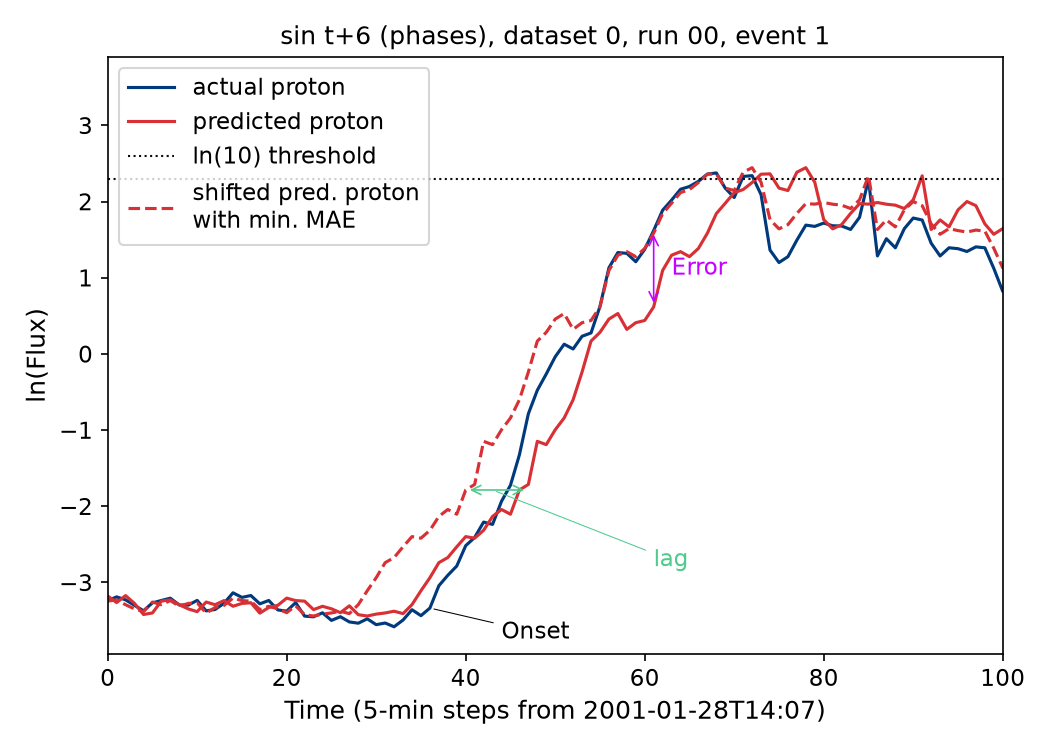
\includegraphics[width=0.7\textwidth,height=0.25\textheight,keepaspectratio]{figs/evaluation/time_intensity_profile/evaluation_criteria/equations/lag_diagram_sin_t+6_phases_dataset0_run00_event1.png}
    \caption{Lag observed on event 1 from sinusoidal transformer.}
    \label{fig:lag_event1}
\end{figure}

\subsubsection{Resampled Block Bootstrapping}

The resample bootstrap is a statistical process that measures the accuracy of our estimated metrics $\hat{\theta}$ with standard
 $\hat{\sigma}$.  With the standard errors we can then approximate confidence intervals of our unknown parameter $\theta$ \cite{Efron1986}. All metrics are computed with
 a $95 \%$ confidence interval.

For a time series, a A block bootstrap partitions the original data and resample the blocks in a shuffled order for a new time series dataset.
A standard bootstrap samples individual timestamps of the fluxes from the original dataset  causing loss of the electron proton rising patterns 
necessary to make predictions.

We first block from $t-36$ before the onset of each event to the end event timestamp and slice them out of the dataset.
This leaves us with the background data left in the time series.
We choose a block size of $N^{1/3}$ where $N$ is the length of our eventless time series data.
\cite{bertail2024optimal}.
Repeating this process nine times plus our original dataset, $d_0$, we are left with ten total datasets. 

\begin{figure}[!htbp]
    \centering
    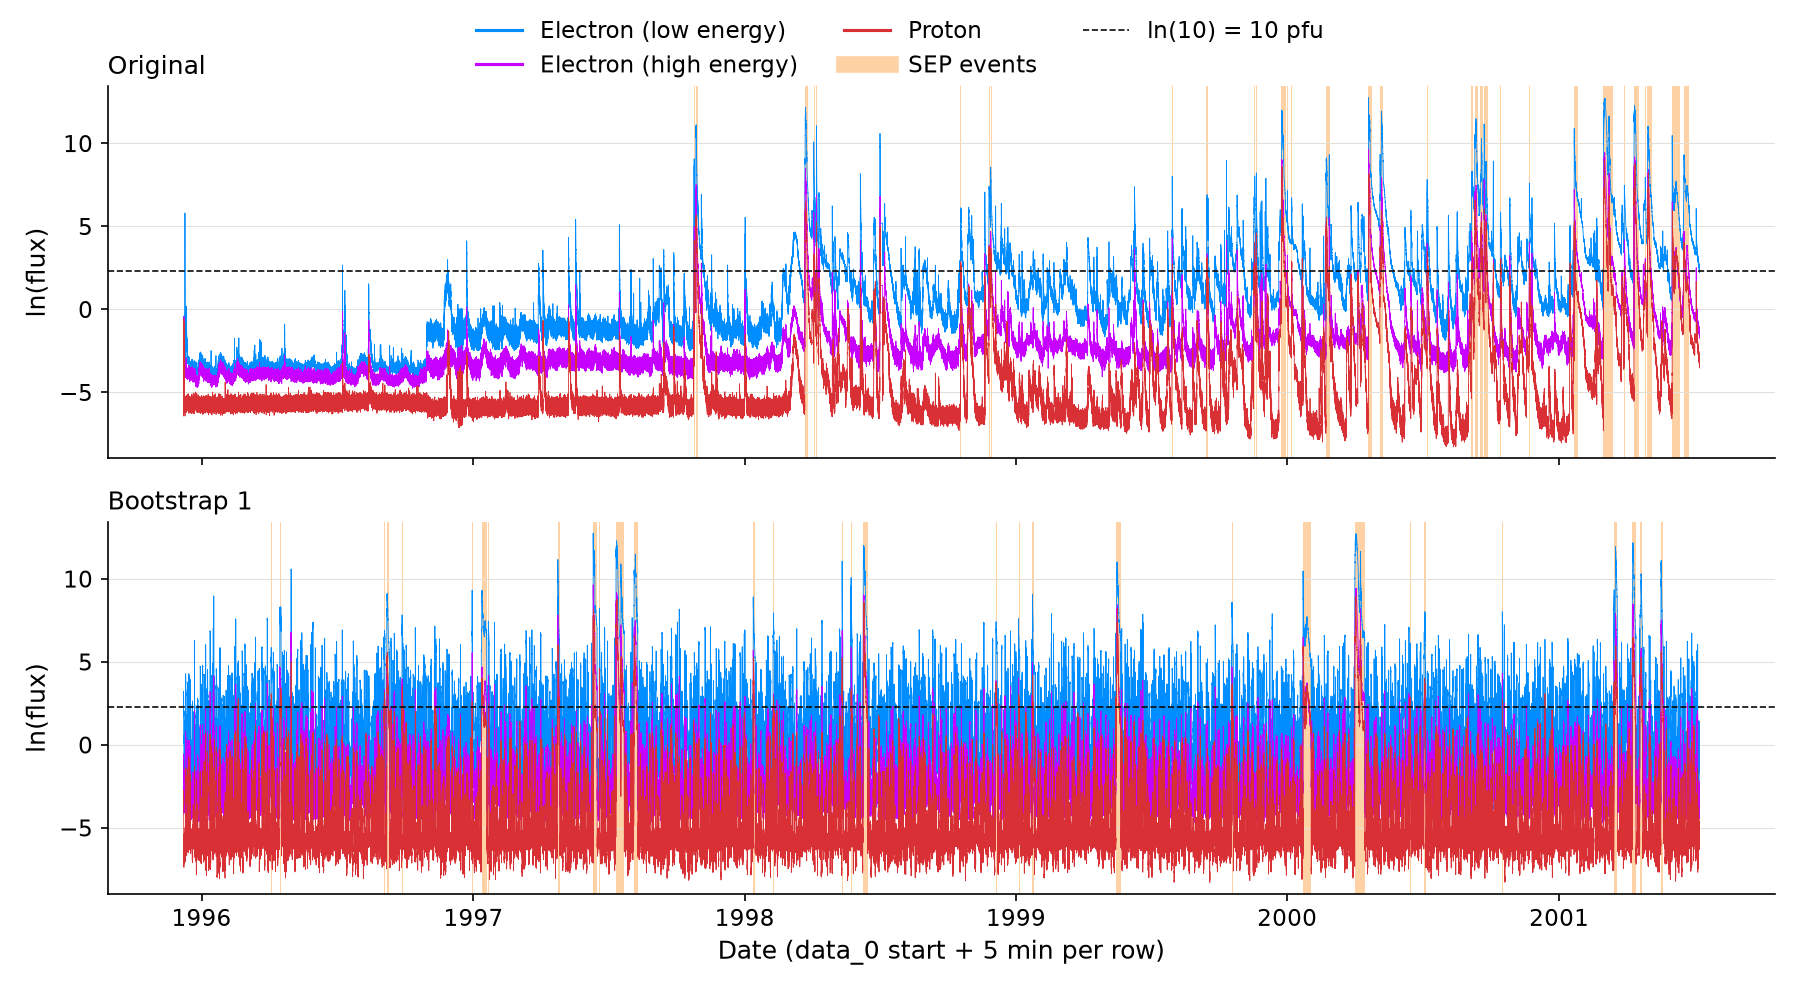
\includegraphics[width=0.9\textwidth,height=0.5\textheight,keepaspectratio]{figs/evaluation/time_intensity_profile/learning_and_evaluation_procedures/equations/bootstrap_stack.png}
    \caption{.}
    \label{fig:bootstrap_chunking}
\end{figure}

Each dataset is split into training and testing portions with an 80/20 ratio. $d_0$ contains $21$ SEP events in the training split and $18$ in the test split.
Bootstrapping randomly switches these events from train or test portions allowing forecasting models learn from all $39$ SEP events rather than $21$.
Each machine learning model trains 10 models on each dataset totaling 100 models for one forecasting time lead $(t+6, t+12)$.

For each model and each dataset we produce a sample, $\theta^*$ of every metric (MAE, Lag, F1, PE). We assume a Student-T distribution for a  small sample size ($n=10$) and unknown population variance. We compute mean estimates for all samples to get a bootstrap estimate of a metric $\hat{\theta}$:
\begin{align*}
    \hat{\theta}^* = \frac{1}{n} \sum_i^n \theta_i^* = \bar{\theta}^*
\end{align*}


For each metric measured from a model trained on a dataset we compute the mean bootstrap estimate

\begin{equation*}
    \bar{\theta} = \frac{1}{B}\sum_i^B \hat{\theta}_i^*
\end{equation*}


Where $B$ is the number of datasets. We retrieve the standard error for  and the standard bias respectively:
\begin{align*}
    S_{\hat{\theta}}^2 = \frac{1}{B-1} \sum_i^B (\hat{\theta}_i^* - \bar{\theta}^*) ^2\
    &&S_{b}^2 = \frac{1}{B} \sum_i^B (\hat{\theta}_i^* - \bar{\theta}^*) ^2
\end{align*}


A bootstrap confidence is calculated with a significance level of $\alpha = .05$:
\begin{align*}
    CI = \left(\bar{\theta} - t_{1-\alpha/2, v} \frac{s_{\theta^*}}{\sqrt{n}} , \bar{\theta} + t_{1-\alpha/2, v}  \frac{s_{\theta^*}}{\sqrt{n}} \right)
\end{align*}

where $v$ is the degrees of freedom and $s_{\theta^*}$ is the sample variance of the bootrap estimate:
\begin{align*}
    s_{\theta^*}^2 = \frac{1}{n}\sum_{i=1}^n (\theta^*_i - \bar{\theta}^*)^2
\end{align*}
 For every deep learning "champion" model we want to compare our metrics with baseline models described in Section~\ref{sec: baseline_methods_used_for_comparison}. A Welch -T Test compares the mean performance of each champion model to baseline model. Neither the population variances are known making this test the most fitting method \cite{delacre2017welch}. We don't expect 
 baseline and champion models to have homogenous variances \cite{welch1947generalization}.
 \begin{align*}
    \text{t-stat} = \frac{(\bar{x}_{simple} - \bar{x}_\text{ML}) - (\mu_{simple} - \mu_\text{ML})}{\sqrt{\frac{s_{\text{simple}}^2}{n_\text{simple}}+\frac{s_{\text{ML}}^2}{n_\text{ML}}}}
\end{align*}


The associated alternative hypothesis tests for each metric is as follows:
\begin{align*}
    H_0 \text{ F1}: \mu_c &\leq \mu_b &&
    H_0 \text{ PE}: \mu_c \leq \mu_b\\
    H_0 \text{ Lag}: |\mu_c| &\geq |\mu_b|&&
    H_0 \text{ MAE}: \mu_c \leq \mu_b
\end{align*}


The Welch-T test does not test the variances of the sample metrics \cite{welch1947generalization}. The Levenes test has been used to measure the spread of samples \cite{zhou2023homogeneity}.
\begin{align*}
    H_0&: \sigma_\text{champ}^2 \geq \sigma_\text{base}^2 \\
    z_i &= \left|\hat{\theta}_i^* - \tilde{\theta}^*\right|\\[6pt]
    \bar{z} &= \frac{1}{B}\sum_i^B z_i\\[6pt]
    S_p^2 &= \frac{S_{z,\text{base}}^2 + S_{z,\text{champ}}^2}{2}\\[6pt]
    t &= \frac{\bar{z}_\text{base} - \bar{z}_\text{champ}}{S_p\sqrt{2/B}}, \qquad v = 2B - 2
\end{align*}



\clearpage
\section{Results}
\label{sec:results}
Figure \ref{fig:rq1_box_mae_nophases} shows the distribution of MAE values on a box and whisker plot for each 
bootstrap dataset. Each model has a set of estimates for both $t+6$ and $t+12$.  The solid bold vertical line indicates the 
median MAE for $t+6$ and the dashed line is for $t+12$. these serve as our benchmarks for our other models to beat. Depending on the metric,
a value larger or smaller could indicate an improvement. At the bottom of the plot is an arrow that points in the direction of improvement. For 
MAE, a smaller value is desirable.
\begin{figure}[H]
    \centering
    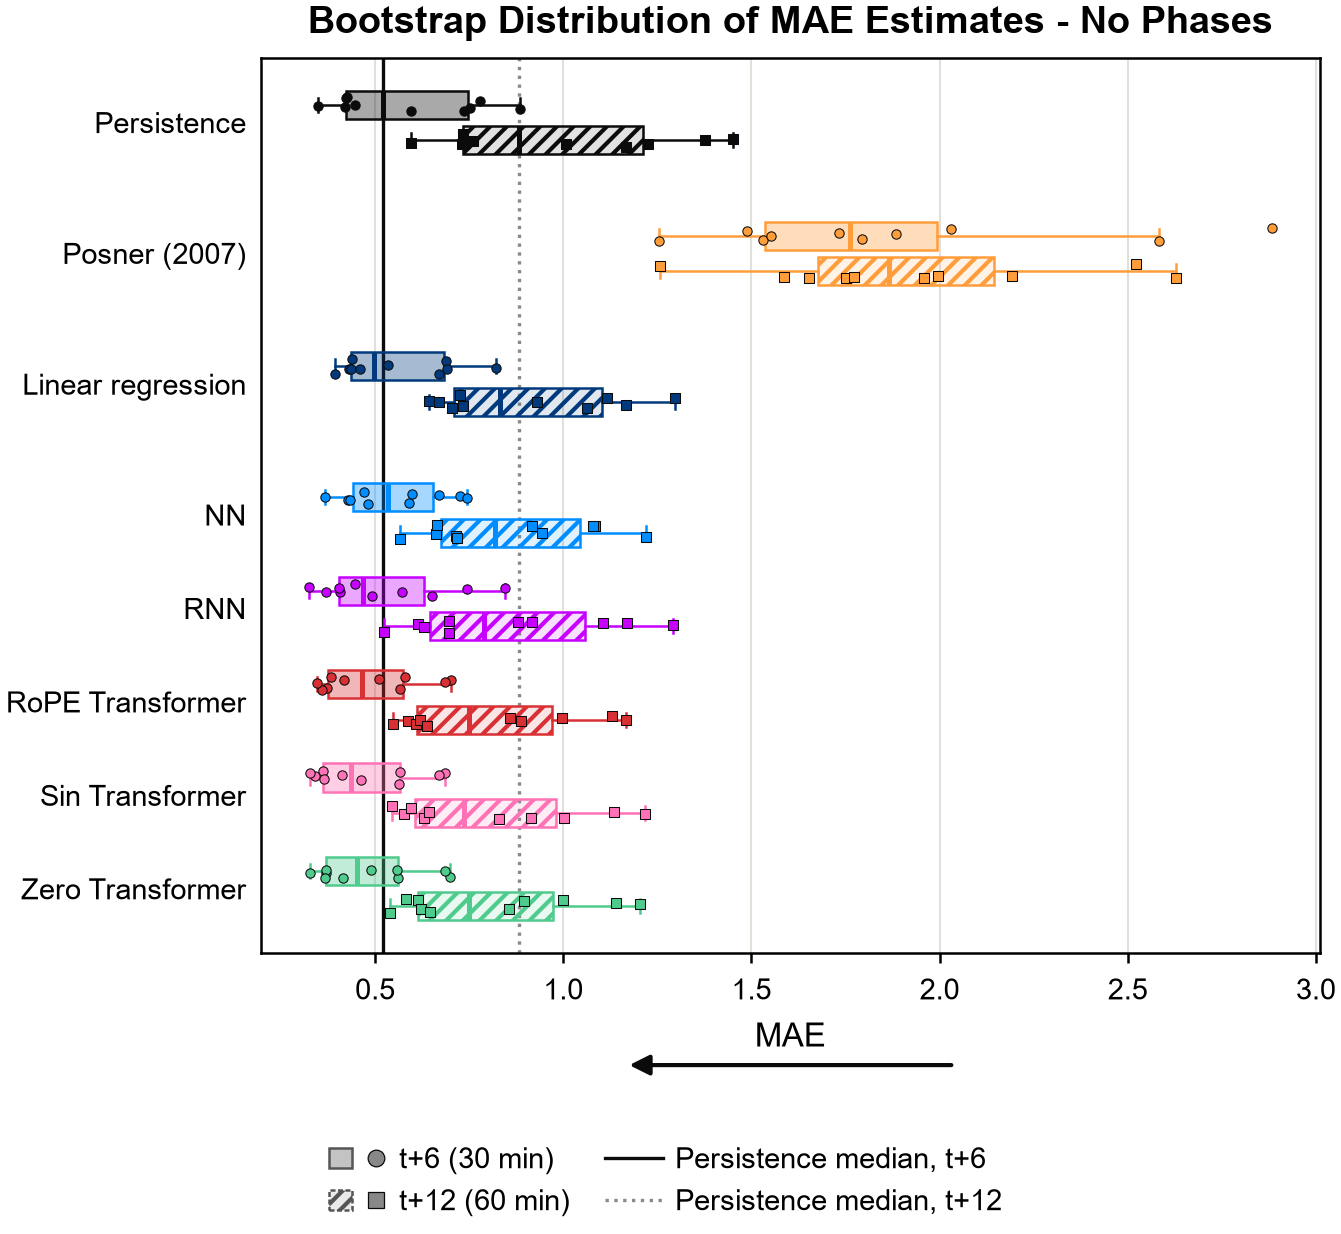
\includegraphics[width=0.8\textwidth,height=0.6\textheight,keepaspectratio]{figs/results/rq1/rq1_box_mae_nophases.png}
    \caption{Bootstrap distributions of MAE for every model without phases. Each marker is the estimate from one of the $B = 10$ bootstrap datasets. Solid boxes and circles are the $t+6$ (30-minute) forecasts, and hatched boxes and squares are the $t+12$ (60-minute) forecasts. The solid and dotted vertical lines are the persistence medians at $t+6$ and $t+12$. The arrow points in the direction of better performance (lower MAE).}
    \label{fig:rq1_box_mae_nophases}
\end{figure}

We can then analyze our results for all metrics in Figure \ref{fig:rq1_box_mae_nophases} for results using no phases, and Figure \ref{fig:rq1_box_phases} for phases.
\begin{figure}[H]
    \centering
    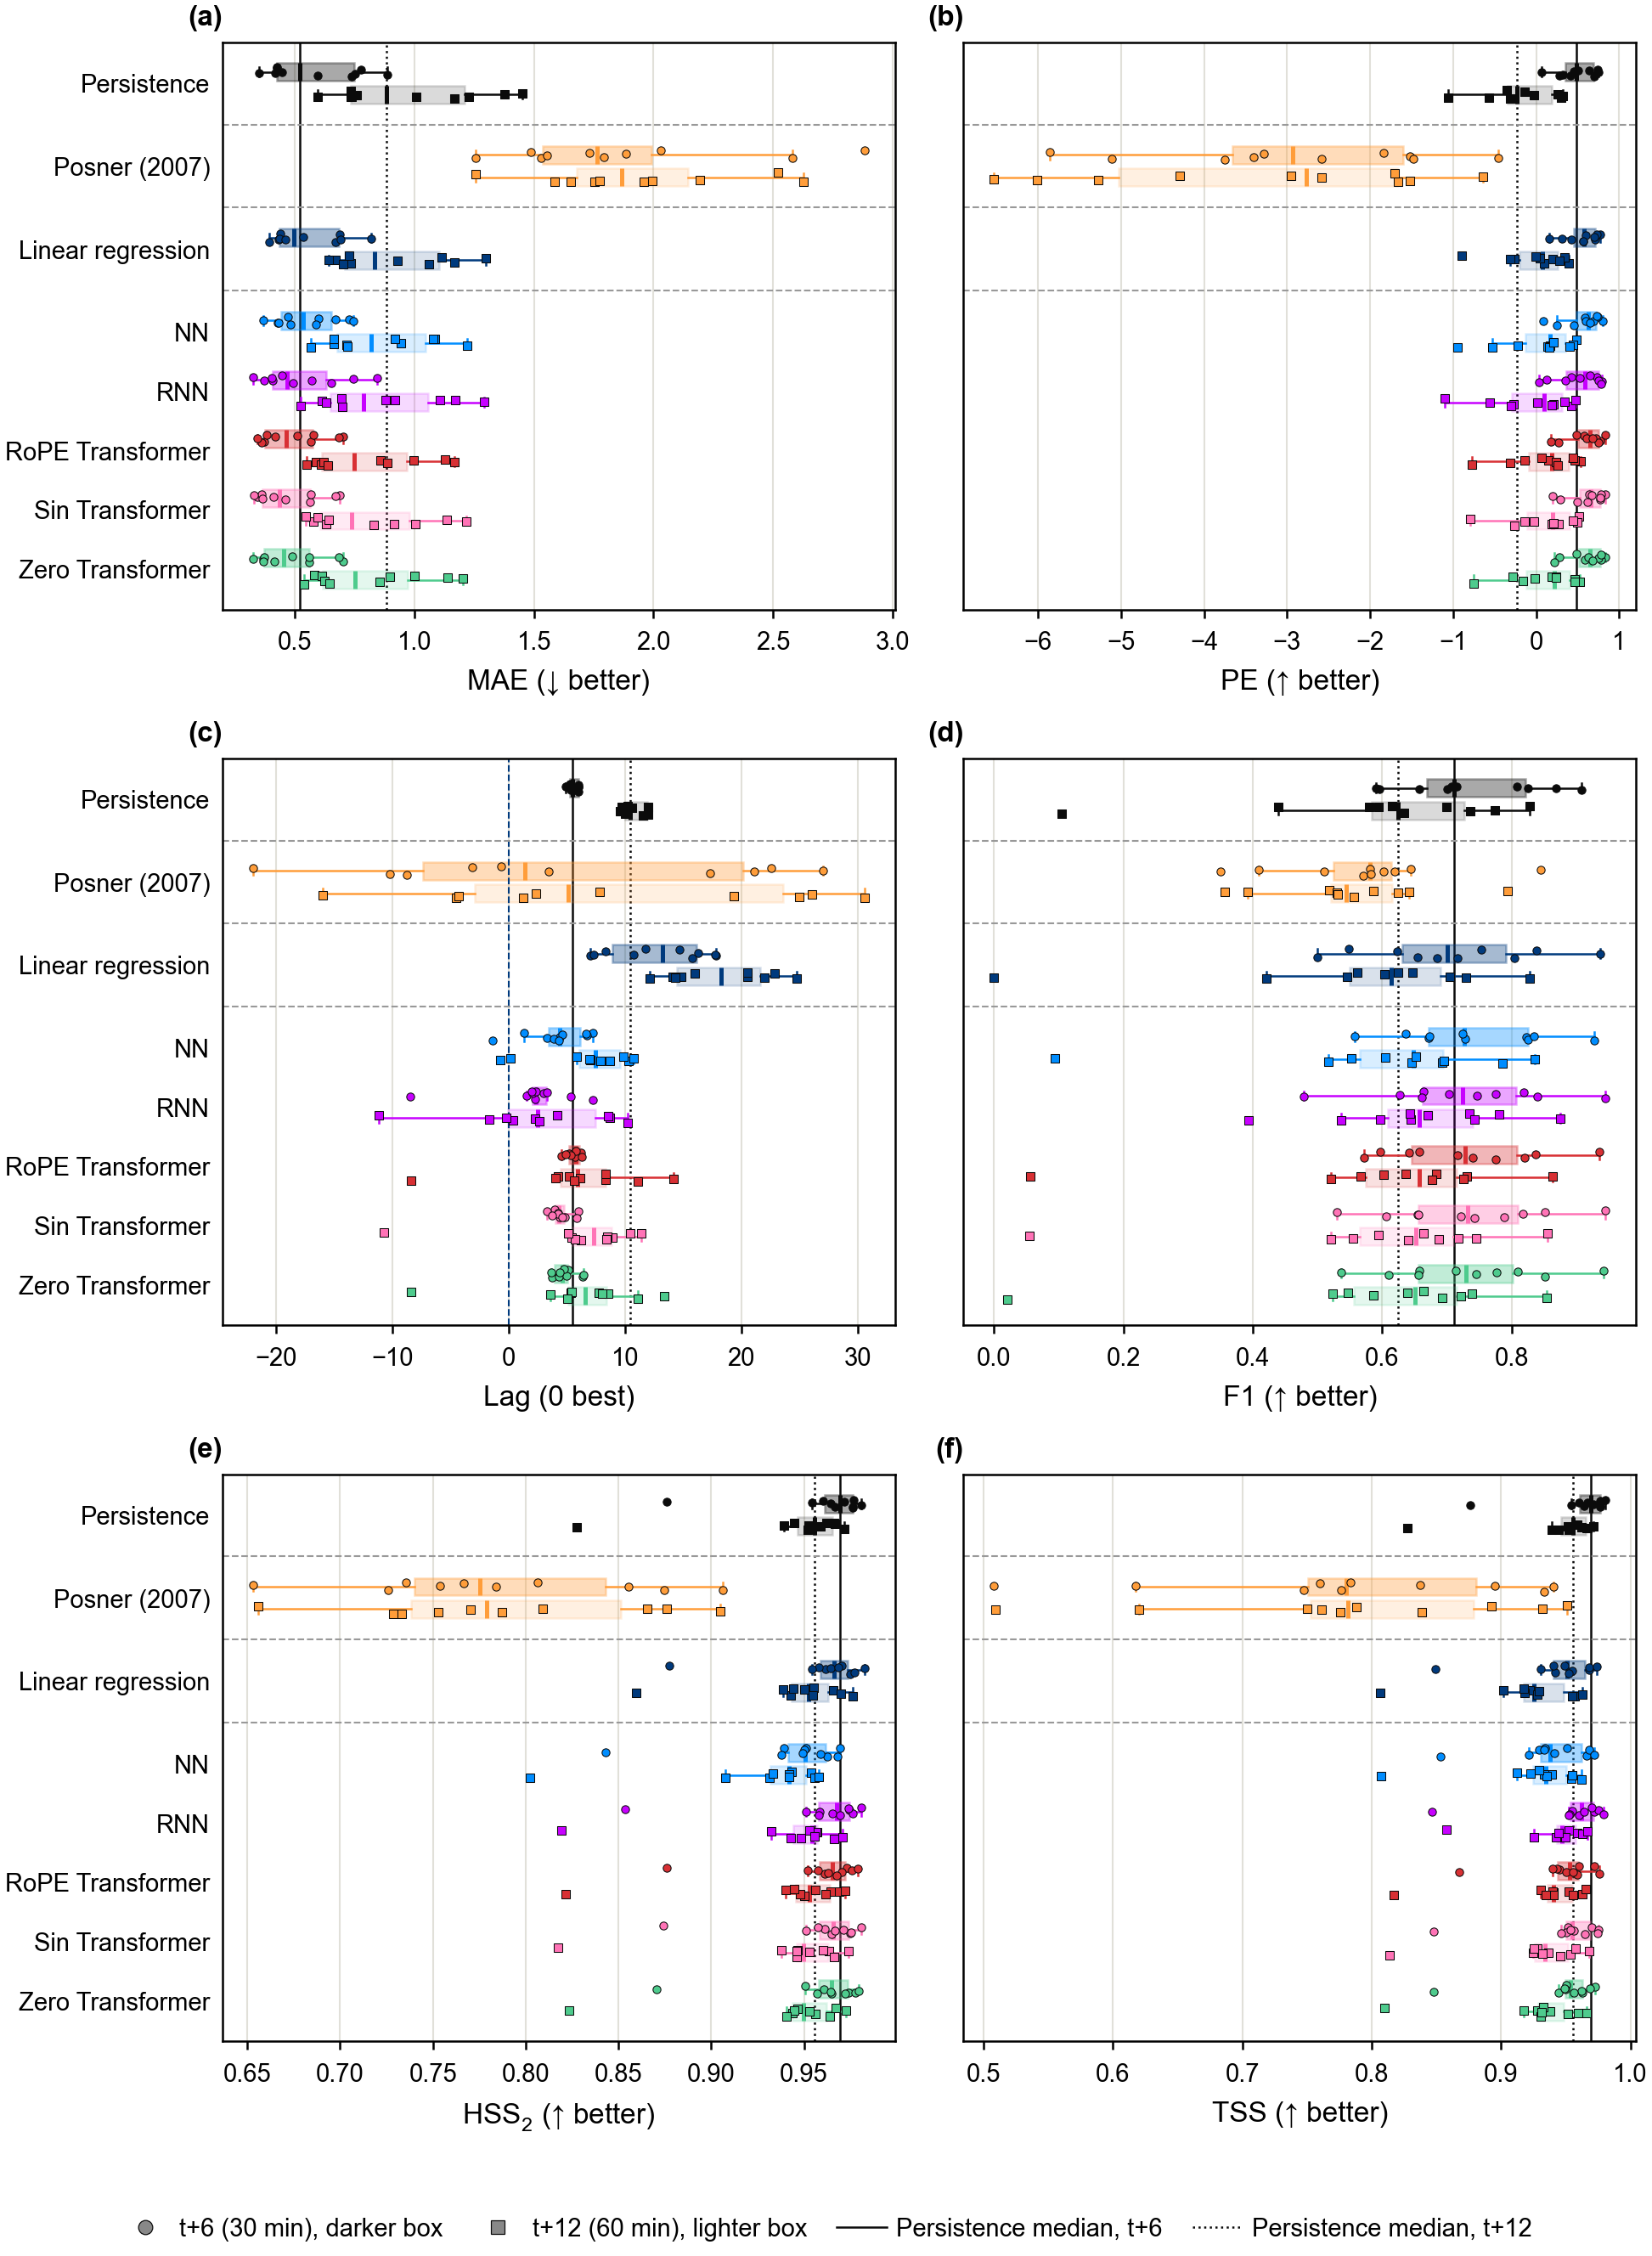
\includegraphics[width=\textwidth,height=0.85\textheight,keepaspectratio]{figs/results/rq1/rq1_box_nophases.png}
    \caption{Bootstrap distributions of (a) MAE, (b) PE, (c) lag, (d) F1, (e) HSS$_2$, and (f) TSS for every model without phases. Each marker is the estimate from one of the $B = 10$ bootstrap datasets. Solid boxes and circles are the $t+6$ (30-minute) forecasts, and hatched boxes and squares are the $t+12$ (60-minute) forecasts. The solid and dotted vertical lines are the persistence medians at $t+6$ and $t+12$. Arrows below each panel point in the direction of better performance; for lag, better is closer to zero.}
    \label{fig:rq1_box_nophases}
\end{figure}

\begin{figure}[H]
    \centering
    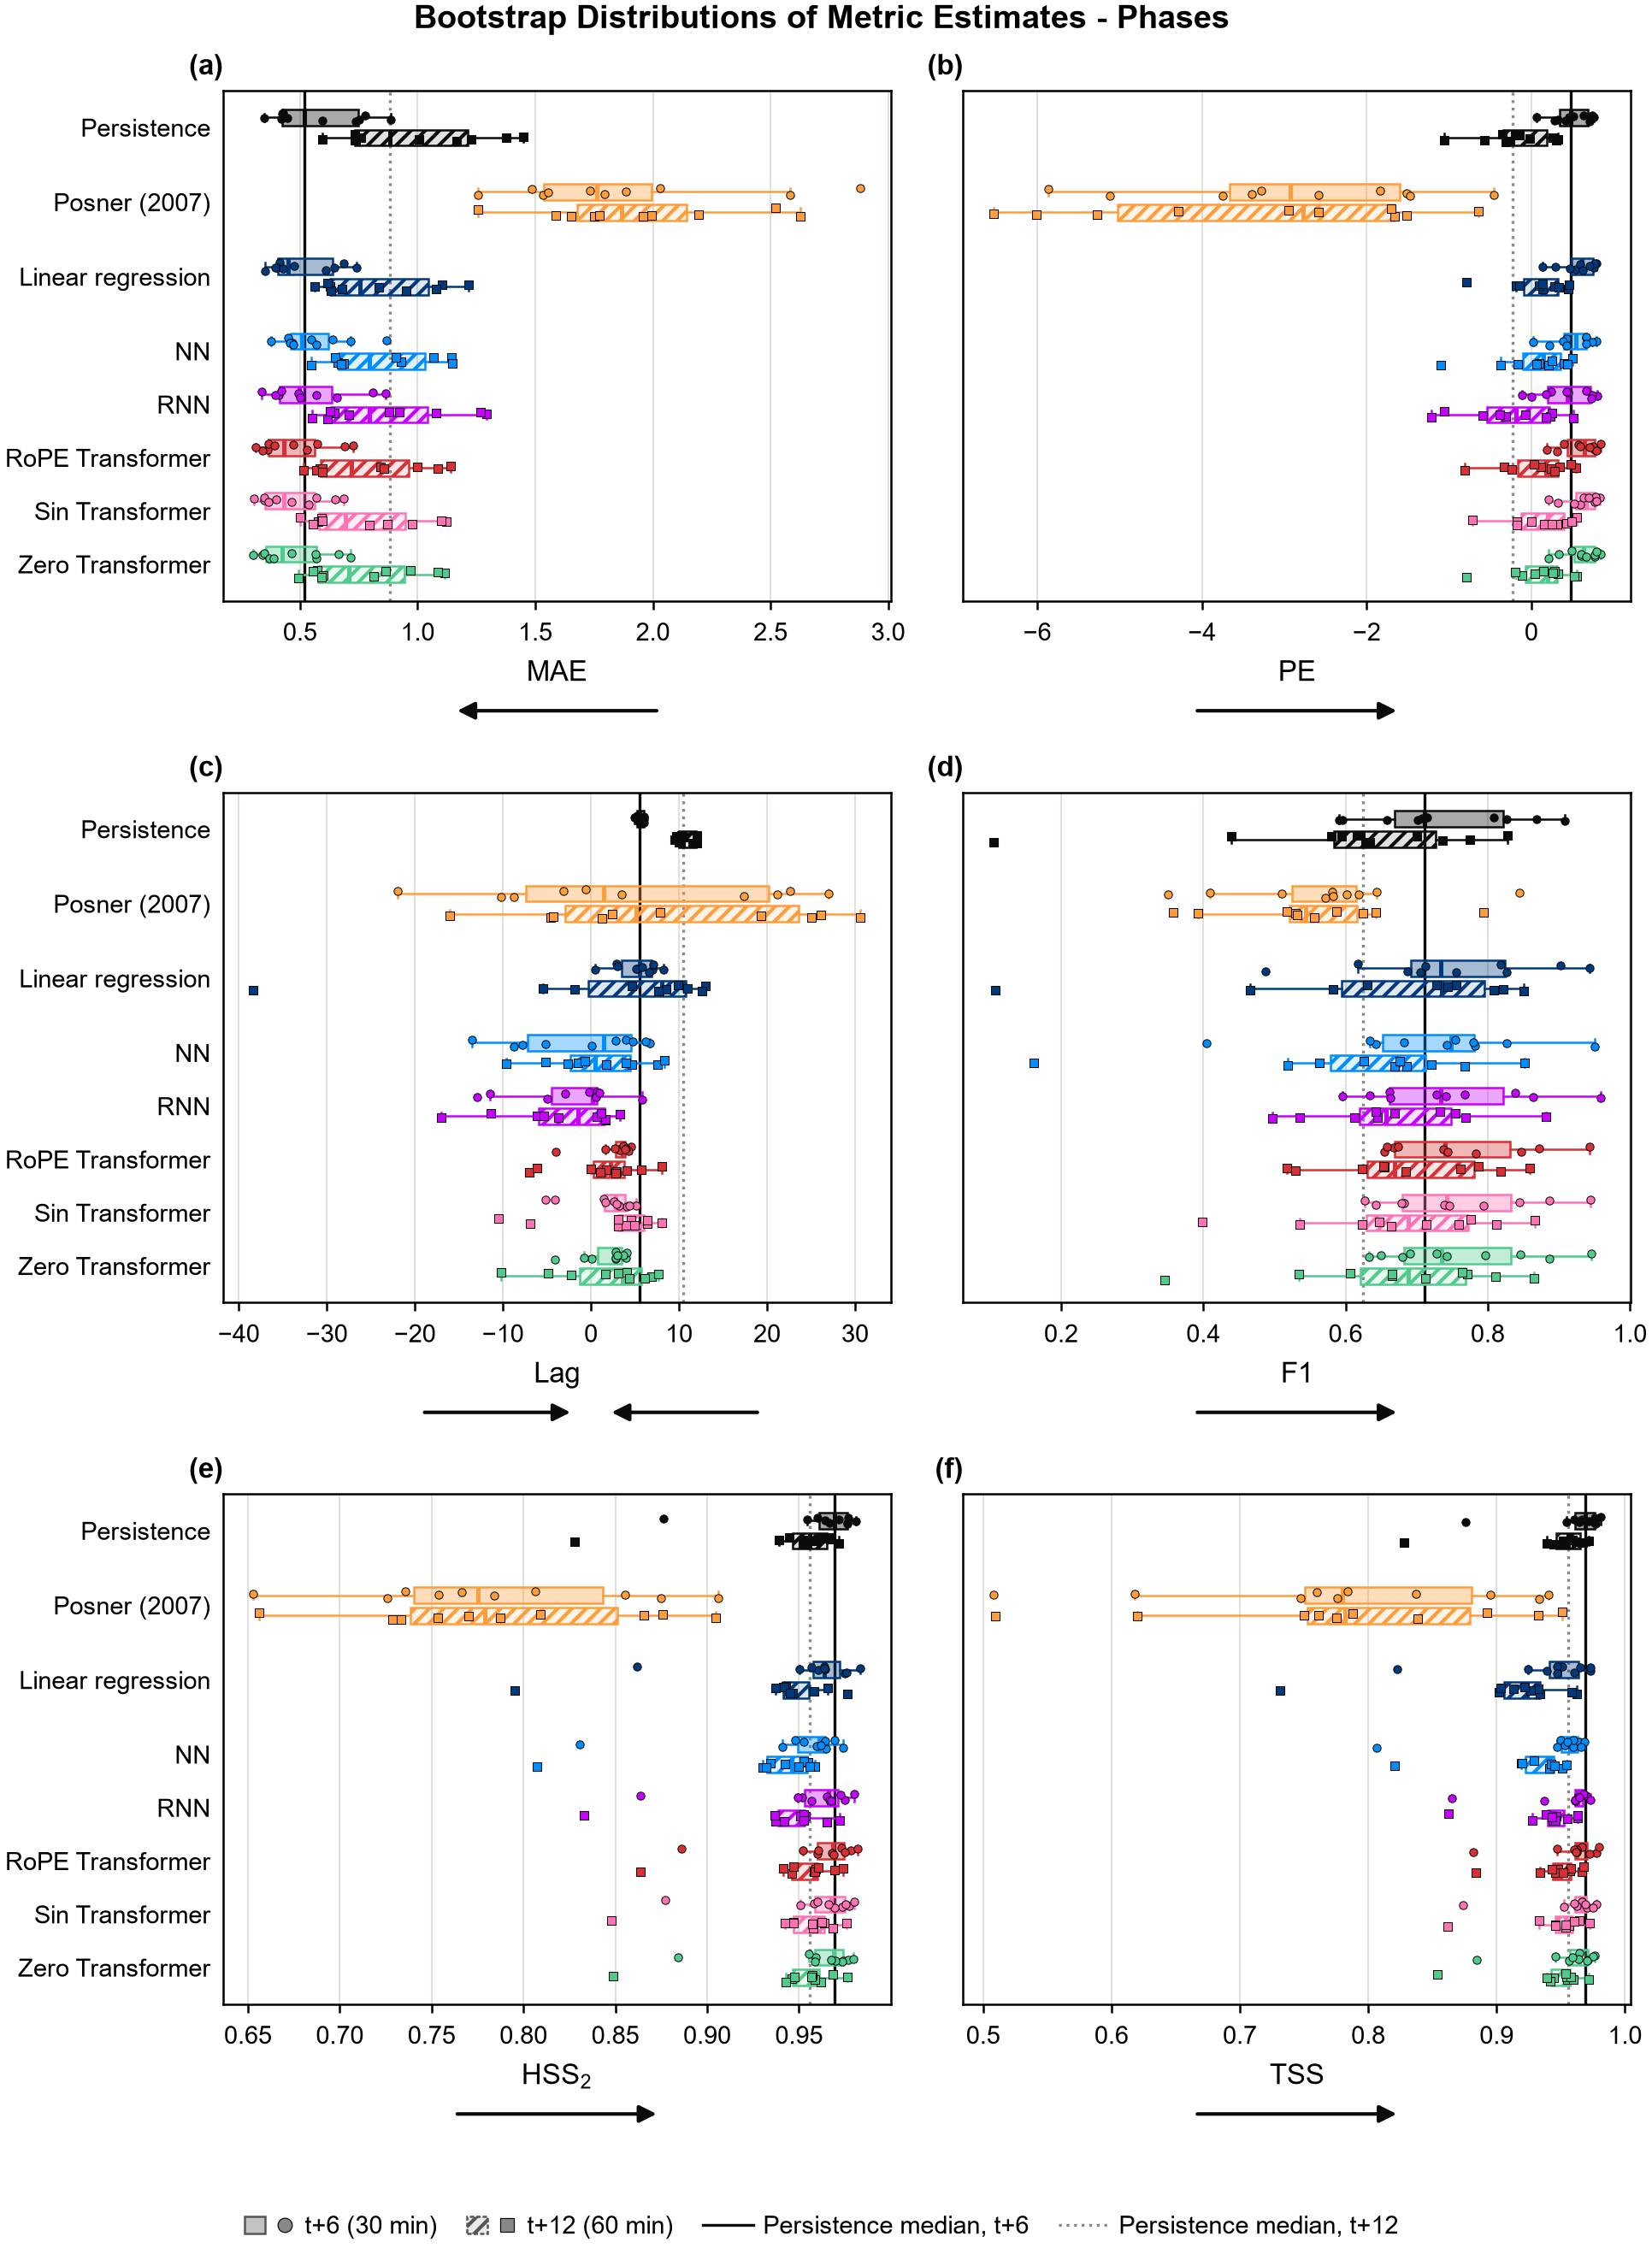
\includegraphics[width=\textwidth,height=0.85\textheight,keepaspectratio]{figs/results/rq1/rq1_box_phases.png}
    \caption{Bootstrap distributions of (a) MAE, (b) PE, (c) lag, (d) F1, (e) HSS2, and (f) TSS for every model with phases. Each marker is the estimate from one of the $B = 10$ bootstrap datasets. Solid boxes and circles are the $t+6$ (30-minute) forecasts, and hatched boxes and squares are the $t+12$ (60-minute) forecasts. The solid and dotted vertical lines are the persistence medians at $t+6$ and $t+12$. Arrows below each panel point in the direction of better performance; for lag, better is closer to zero.}
    \label{fig:rq1_box_phases}
\end{figure}

A common feature across all metrics is the Posner model underperforming in forecasting SEPs. \citeA{torres2025machine} demonstrates the same disparity 
for the MAE values. The min and max values on the Posner plots are much further apart than all other models which indicates an
unreliability in the model. Posner was explained to have overpredicted SEP events causing a lower lag value \cite{torres2025machine}, but over multiple bootstrap runs, 
that advantage disappears.

Over the distribution all other models  appears to perform relatively equivalent to the persistence model. Despite the complex regressive training from the machine learning models a nowcast of the proton flux is 
indistinguishable. The parameter size of the models and the limited SEP event dataset 
play a role in the model performance. Table \ref{tab:rq1_box} displays the bootstrap mean and standard error of all metrics.    
Bold values are the best mean metric results in that category.

\begin{table}[H]
\centering
\definecolor{nophasesbest}{HTML}{C701FF}
\definecolor{phasesbest}{HTML}{008DFF}
\caption{Mean bootstrap metric estimates with bootstrap standard errors. A purple value indicates the best value of that metric observed from a model for no phases while blue is for phases. Scores that tie with each other are both highlighted}
\label{tab:rq1_box}
\resizebox{\textwidth}{!}{%
\begin{tabular}{lllrrrrrr}
\toprule
Model & Input & Horizon & MAE & PE & Lag & F1 & HSS$_2$ & TSS \\
\midrule
Persistence & No Phases & $t+6$ & $0.58$ $(0.19)$ & $0.49$ $(0.23)$ & $5.5$ $(0.4)$ & $\textcolor{nophasesbest}{\mathbf{0.74}}$ $(0.11)$ & $\textcolor{nophasesbest}{\mathbf{0.96}}$ $(0.03)$ & $\textcolor{nophasesbest}{\mathbf{0.96}}$ $(0.03)$ \\
 &  & $t+12$ & $0.98$ $(0.31)$ & $-0.19$ $(0.43)$ & $10.8$ $(1.0)$ & $0.60$ $(0.21)$ & $0.94$ $(0.04)$ & $\textcolor{nophasesbest}{\mathbf{0.94}}$ $(0.04)$ \\
\ifdefined\arrayrulecolor\arrayrulecolor{gray!50}\fi\cmidrule[0.4pt](lr){2-9}\ifdefined\arrayrulecolor\arrayrulecolor{black}\fi
 & Phases & $t+6$ & $0.58$ $(0.19)$ & $0.49$ $(0.23)$ & $5.5$ $(0.4)$ & $0.74$ $(0.11)$ & $\textcolor{phasesbest}{\mathbf{0.96}}$ $(0.03)$ & $\textcolor{phasesbest}{\mathbf{0.96}}$ $(0.03)$ \\
 &  & $t+12$ & $0.98$ $(0.31)$ & $-0.19$ $(0.43)$ & $10.8$ $(1.0)$ & $0.60$ $(0.21)$ & $0.94$ $(0.04)$ & $0.94$ $(0.04)$ \\
\midrule
Posner (2007) & No Phases & $t+6$ & $1.87$ $(0.51)$ & $-2.93$ $(1.70)$ & $4.7$ $(16.5)$ & $0.57$ $(0.13)$ & $0.79$ $(0.08)$ & $0.78$ $(0.14)$ \\
 &  & $t+12$ & $1.93$ $(0.42)$ & $-3.32$ $(2.08)$ & $8.8$ $(15.7)$ & $0.55$ $(0.12)$ & $0.79$ $(0.08)$ & $0.78$ $(0.14)$ \\
\ifdefined\arrayrulecolor\arrayrulecolor{gray!50}\fi\cmidrule[0.4pt](lr){2-9}\ifdefined\arrayrulecolor\arrayrulecolor{black}\fi
 & Phases & $t+6$ & $1.87$ $(0.51)$ & $-2.93$ $(1.70)$ & $4.7$ $(16.5)$ & $0.57$ $(0.13)$ & $0.79$ $(0.08)$ & $0.78$ $(0.14)$ \\
 &  & $t+12$ & $1.93$ $(0.42)$ & $-3.32$ $(2.08)$ & $8.8$ $(15.7)$ & $0.55$ $(0.12)$ & $0.79$ $(0.08)$ & $0.78$ $(0.14)$ \\
\midrule
Linear regression & No Phases & $t+6$ & $0.56$ $(0.15)$ & $0.55$ $(0.20)$ & $12.8$ $(4.3)$ & $0.71$ $(0.13)$ & $\textcolor{nophasesbest}{\mathbf{0.96}}$ $(0.03)$ & $0.94$ $(0.04)$ \\
 &  & $t+12$ & $0.90$ $(0.24)$ & $-0.01$ $(0.39)$ & $18.2$ $(4.4)$ & $0.57$ $(0.23)$ & $\textcolor{nophasesbest}{\mathbf{0.95}}$ $(0.03)$ & $0.92$ $(0.04)$ \\
\ifdefined\arrayrulecolor\arrayrulecolor{gray!50}\fi\cmidrule[0.4pt](lr){2-9}\ifdefined\arrayrulecolor\arrayrulecolor{black}\fi
 & Phases & $t+6$ & $0.51$ $(0.14)$ & $0.57$ $(0.22)$ & $5.1$ $(2.4)$ & $0.75$ $(0.14)$ & $\textcolor{phasesbest}{\mathbf{0.96}}$ $(0.03)$ & $0.94$ $(0.04)$ \\
 &  & $t+12$ & $0.83$ $(0.24)$ & $0.08$ $(0.37)$ & $2.2$ $(15.5)$ & $0.65$ $(0.22)$ & $0.94$ $(0.05)$ & $0.91$ $(0.07)$ \\
\midrule
NN & No Phases & $t+6$ & $0.55$ $(0.13)$ & $0.56$ $(0.23)$ & $4.1$ $(2.6)$ & $\textcolor{nophasesbest}{\mathbf{0.74}}$ $(0.11)$ & $0.94$ $(0.04)$ & $0.94$ $(0.03)$ \\
 &  & $t+12$ & $0.86$ $(0.22)$ & $0.03$ $(0.46)$ & $6.7$ $(4.0)$ & $0.61$ $(0.20)$ & $0.93$ $(0.05)$ & $0.93$ $(0.04)$ \\
\ifdefined\arrayrulecolor\arrayrulecolor{gray!50}\fi\cmidrule[0.4pt](lr){2-9}\ifdefined\arrayrulecolor\arrayrulecolor{black}\fi
 & Phases & $t+6$ & $0.56$ $(0.15)$ & $0.50$ $(0.25)$ & $\textcolor{phasesbest}{\mathbf{-1.1}}$ $(7.2)$ & $0.72$ $(0.14)$ & $0.95$ $(0.04)$ & $0.94$ $(0.05)$ \\
 &  & $t+12$ & $0.84$ $(0.23)$ & $0.03$ $(0.48)$ & $\textcolor{phasesbest}{\mathbf{0.7}}$ $(5.7)$ & $0.62$ $(0.19)$ & $0.93$ $(0.04)$ & $0.93$ $(0.04)$ \\
\midrule
RNN & No Phases & $t+6$ & $0.53$ $(0.17)$ & $0.52$ $(0.27)$ & $\textcolor{nophasesbest}{\mathbf{2.1}}$ $(4.1)$ & $0.73$ $(0.13)$ & $\textcolor{nophasesbest}{\mathbf{0.96}}$ $(0.04)$ & $0.95$ $(0.04)$ \\
 &  & $t+12$ & $0.85$ $(0.26)$ & $-0.06$ $(0.50)$ & $\textcolor{nophasesbest}{\mathbf{2.4}}$ $(6.3)$ & $\textcolor{nophasesbest}{\mathbf{0.66}}$ $(0.14)$ & $0.94$ $(0.04)$ & $\textcolor{nophasesbest}{\mathbf{0.94}}$ $(0.03)$ \\
\ifdefined\arrayrulecolor\arrayrulecolor{gray!50}\fi\cmidrule[0.4pt](lr){2-9}\ifdefined\arrayrulecolor\arrayrulecolor{black}\fi
 & Phases & $t+6$ & $0.55$ $(0.18)$ & $0.41$ $(0.32)$ & $-2.4$ $(5.9)$ & $0.75$ $(0.11)$ & $0.95$ $(0.03)$ & $0.95$ $(0.03)$ \\
 &  & $t+12$ & $0.86$ $(0.28)$ & $-0.24$ $(0.58)$ & $-3.5$ $(6.6)$ & $0.67$ $(0.11)$ & $0.94$ $(0.04)$ & $0.94$ $(0.03)$ \\
\midrule
RoPE & No Phases & $t+6$ & $0.49$ $(0.14)$ & $0.59$ $(0.22)$ & $5.6$ $(0.6)$ & $0.73$ $(0.12)$ & $\textcolor{nophasesbest}{\mathbf{0.96}}$ $(0.03)$ & $0.95$ $(0.03)$ \\
 &  & $t+12$ & $\textcolor{nophasesbest}{\mathbf{0.80}}$ $(0.23)$ & $\textcolor{nophasesbest}{\mathbf{0.09}}$ $(0.41)$ & $5.9$ $(6.0)$ & $0.61$ $(0.22)$ & $0.94$ $(0.04)$ & $0.93$ $(0.04)$ \\
\ifdefined\arrayrulecolor\arrayrulecolor{gray!50}\fi\cmidrule[0.4pt](lr){2-9}\ifdefined\arrayrulecolor\arrayrulecolor{black}\fi
 & Phases & $t+6$ & $0.48$ $(0.15)$ & $0.59$ $(0.22)$ & $2.7$ $(2.5)$ & $\textcolor{phasesbest}{\mathbf{0.76}}$ $(0.10)$ & $\textcolor{phasesbest}{\mathbf{0.96}}$ $(0.03)$ & $\textcolor{phasesbest}{\mathbf{0.96}}$ $(0.03)$ \\
 &  & $t+12$ & $0.78$ $(0.24)$ & $0.07$ $(0.42)$ & $1.3$ $(4.8)$ & $\textcolor{phasesbest}{\mathbf{0.69}}$ $(0.12)$ & $\textcolor{phasesbest}{\mathbf{0.95}}$ $(0.03)$ & $\textcolor{phasesbest}{\mathbf{0.95}}$ $(0.02)$ \\
\midrule
Sinusoidal & No Phases & $t+6$ & $\textcolor{nophasesbest}{\mathbf{0.48}}$ $(0.14)$ & $\textcolor{nophasesbest}{\mathbf{0.61}}$ $(0.22)$ & $4.5$ $(0.9)$ & $0.73$ $(0.12)$ & $\textcolor{nophasesbest}{\mathbf{0.96}}$ $(0.03)$ & $0.95$ $(0.04)$ \\
 &  & $t+12$ & $0.81$ $(0.25)$ & $\textcolor{nophasesbest}{\mathbf{0.09}}$ $(0.41)$ & $5.9$ $(6.2)$ & $0.60$ $(0.22)$ & $0.94$ $(0.04)$ & $0.93$ $(0.04)$ \\
\ifdefined\arrayrulecolor\arrayrulecolor{gray!50}\fi\cmidrule[0.4pt](lr){2-9}\ifdefined\arrayrulecolor\arrayrulecolor{black}\fi
 & Phases & $t+6$ & $\textcolor{phasesbest}{\mathbf{0.47}}$ $(0.14)$ & $\textcolor{phasesbest}{\mathbf{0.61}}$ $(0.21)$ & $1.6$ $(3.5)$ & $\textcolor{phasesbest}{\mathbf{0.76}}$ $(0.11)$ & $\textcolor{phasesbest}{\mathbf{0.96}}$ $(0.03)$ & $\textcolor{phasesbest}{\mathbf{0.96}}$ $(0.03)$ \\
 &  & $t+12$ & $\textcolor{phasesbest}{\mathbf{0.77}}$ $(0.24)$ & $\textcolor{phasesbest}{\mathbf{0.11}}$ $(0.39)$ & $2.3$ $(6.1)$ & $0.68$ $(0.14)$ & $\textcolor{phasesbest}{\mathbf{0.95}}$ $(0.04)$ & $0.94$ $(0.03)$ \\
\midrule
Zero-Init & No Phases & $t+6$ & $\textcolor{nophasesbest}{\mathbf{0.48}}$ $(0.14)$ & $0.60$ $(0.21)$ & $4.8$ $(1.0)$ & $0.73$ $(0.12)$ & $\textcolor{nophasesbest}{\mathbf{0.96}}$ $(0.03)$ & $0.95$ $(0.04)$ \\
 &  & $t+12$ & $0.81$ $(0.24)$ & $\textcolor{nophasesbest}{\mathbf{0.09}}$ $(0.40)$ & $6.0$ $(5.9)$ & $0.60$ $(0.23)$ & $0.94$ $(0.04)$ & $0.93$ $(0.04)$ \\
\ifdefined\arrayrulecolor\arrayrulecolor{gray!50}\fi\cmidrule[0.4pt](lr){2-9}\ifdefined\arrayrulecolor\arrayrulecolor{black}\fi
 & Phases & $t+6$ & $\textcolor{phasesbest}{\mathbf{0.47}}$ $(0.15)$ & $\textcolor{phasesbest}{\mathbf{0.61}}$ $(0.21)$ & $1.8$ $(2.6)$ & $\textcolor{phasesbest}{\mathbf{0.76}}$ $(0.11)$ & $\textcolor{phasesbest}{\mathbf{0.96}}$ $(0.03)$ & $\textcolor{phasesbest}{\mathbf{0.96}}$ $(0.03)$ \\
 &  & $t+12$ & $\textcolor{phasesbest}{\mathbf{0.77}}$ $(0.23)$ & $0.10$ $(0.40)$ & $1.7$ $(5.7)$ & $0.67$ $(0.15)$ & $\textcolor{phasesbest}{\mathbf{0.95}}$ $(0.04)$ & $0.94$ $(0.03)$ \\
\bottomrule
\end{tabular}%
}
\end{table}

To make a definitive statement on the effectiveness of the forecasting models, Figure \ref{fig:rq1_welch} shows the results of a one sided $t$ test. Each box is colored either red or green to indicate whether the model 
performs on average better than persistence.The values inside are the reported $p$ values.
\begin{figure}[H]
    \centering
    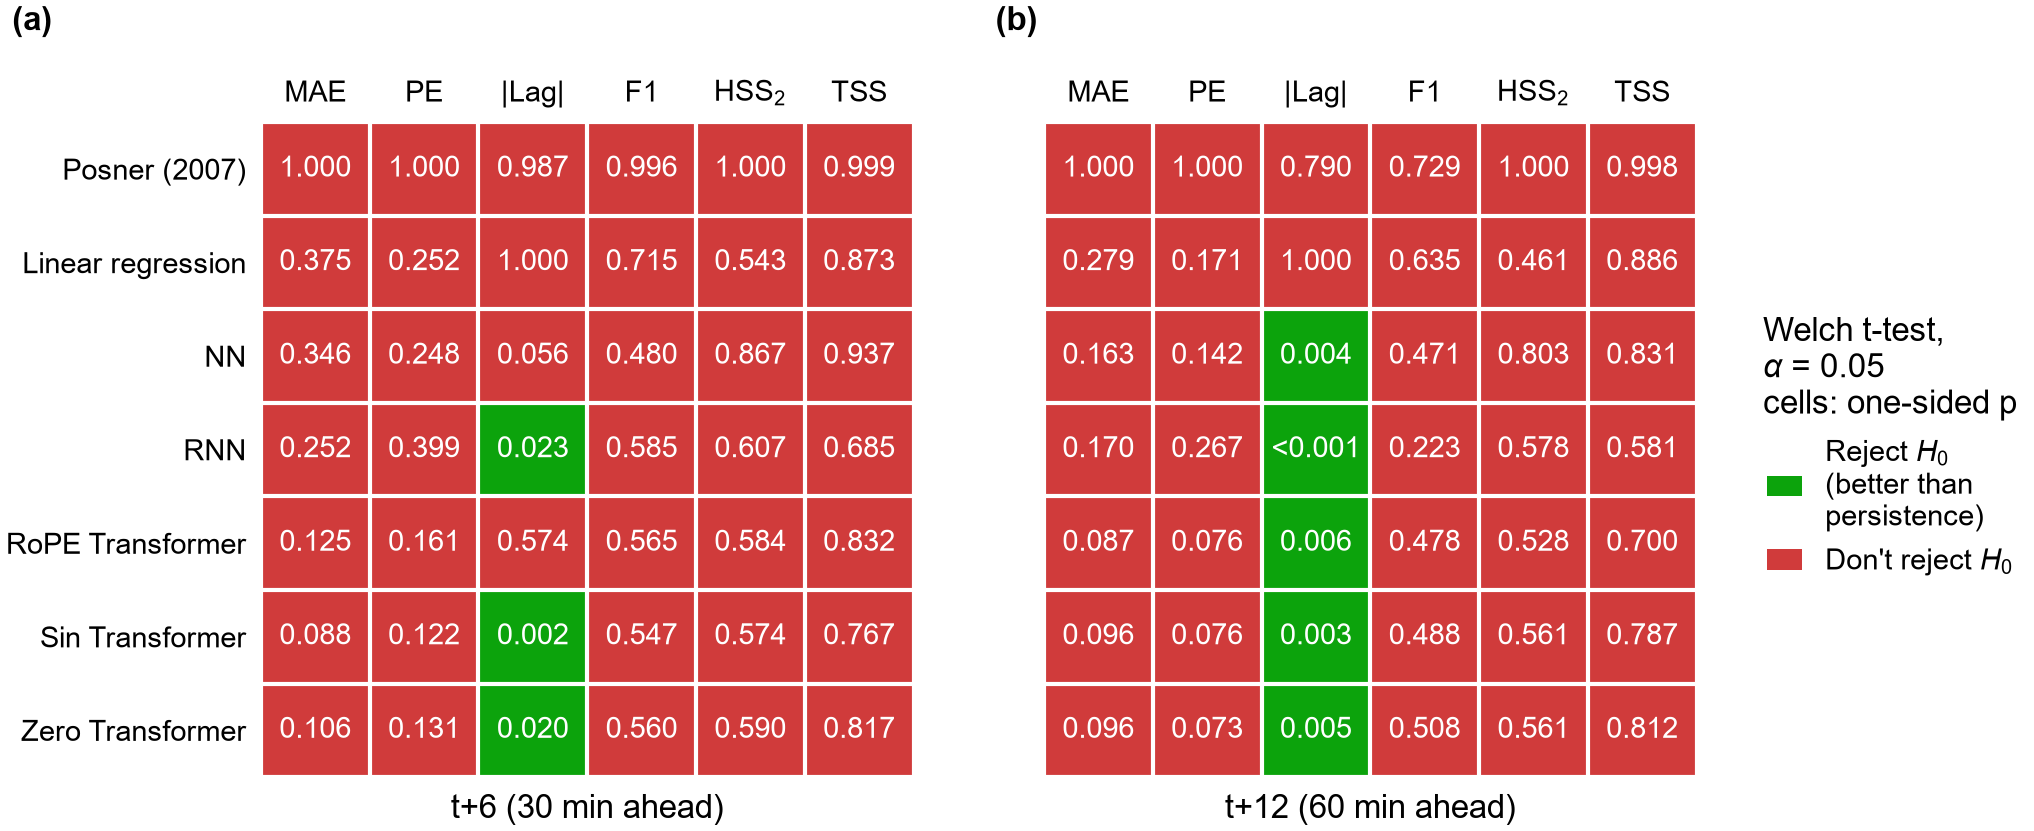
\includegraphics[width=\textwidth,keepaspectratio]{figs/results/rq1/rq1_welch_nophases.png}
    \caption{One-sided $p$-values from Welch's $t$-test: No-Phases}
    \label{fig:rq1_welch_nophases}
\end{figure}


All models hardly ever beat persistence. Posner $p$ value is always $\approx$ 1.00 which indicates it's significantly worse.
The only advantage some models have is lag.

\begin{figure}[H]
    \centering
    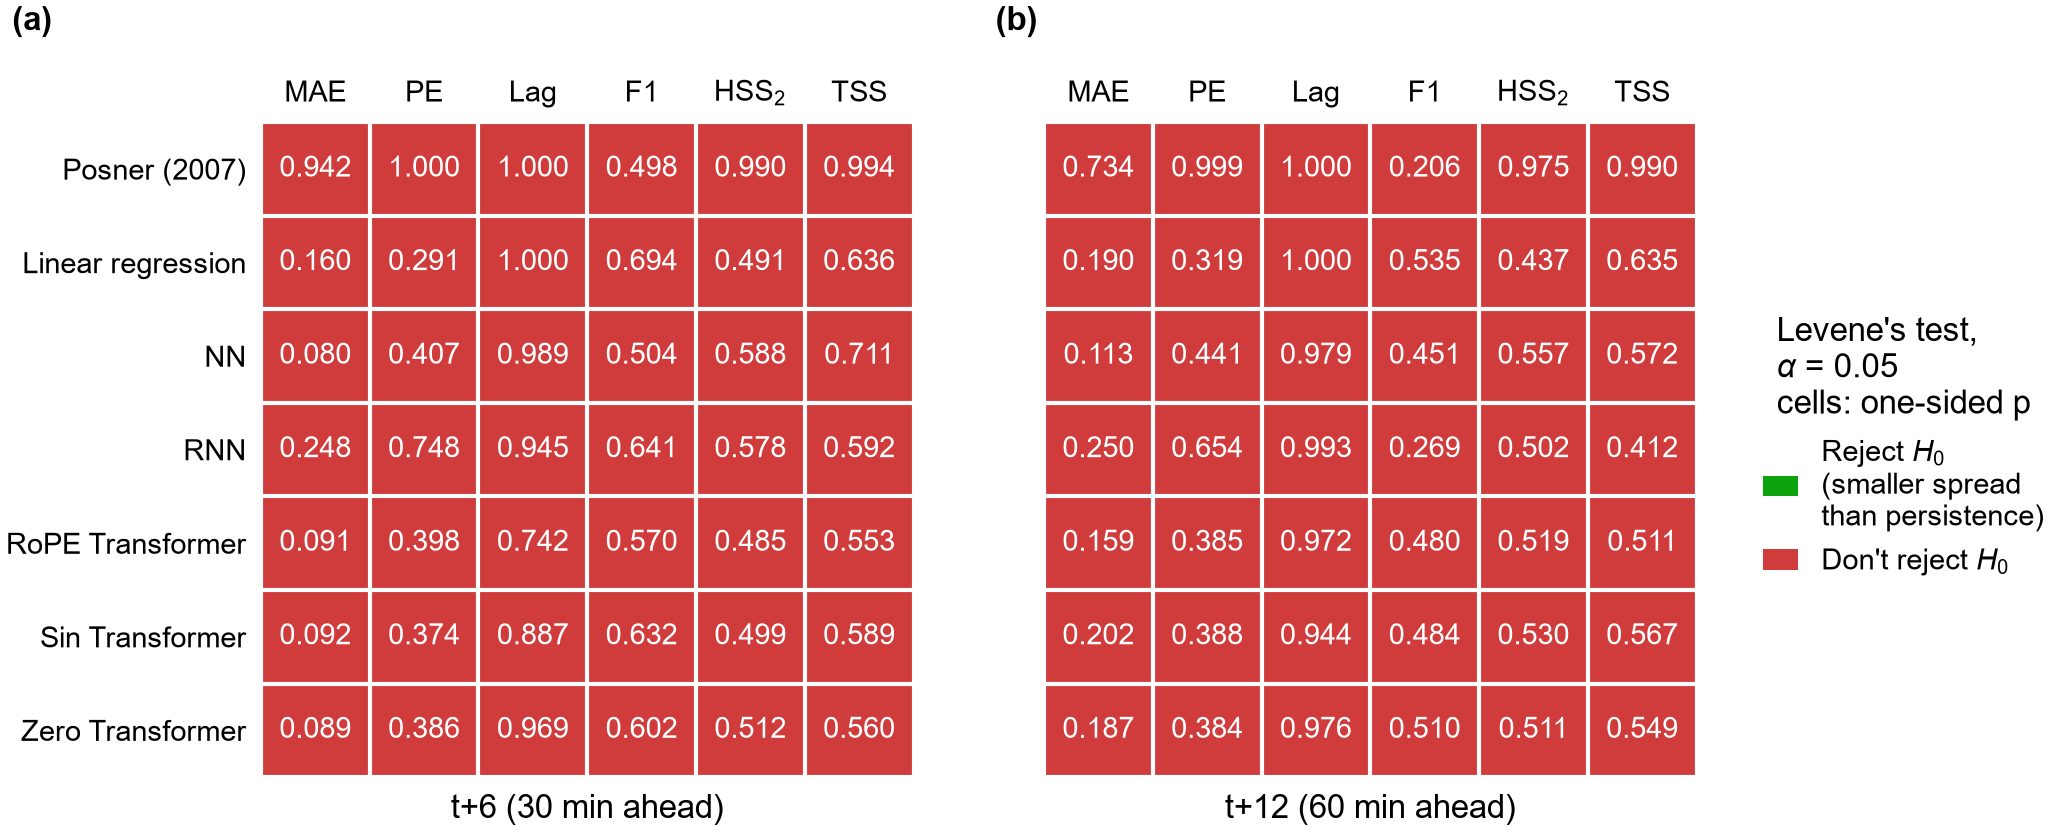
\includegraphics[width=\textwidth,keepaspectratio]{figs/results/rq1/rq1_levene_nophases.png}
    \caption{One-sided $p$-values from Levene's test: No-Phases}
    \label{fig:rq1_levene_nophases}
\end{figure}

no model is more consistent than persistence cause they suck.
\clearpage
\section{Conclusion}
\label{sec:conclusion}
Our goal was to build a series of time series transformers to improve the forecasting of SEPs. We built three time series transformers to compete with previous models.
We compared our metrics to those of previous models and found little change relative not only to the physics and empirical models,
but also to the persistence model. MSE, MAE, F1, PE, $\text{HSS}_2$, and TSS were shown to be reliably better for the persistence model, even though all other models had better raw bootstrap mean scores across.
The other models were able to reduce the lag time between predicted and true protons.

The positional encodings within the transformer models also made no difference, indicating a low correlation with effective SEP forecasting. Improvements can be made by scaling the complexity of our models while also adding more context
to the input window through a length generalization study.

\subsection{Future Work}
The machine learning models trained in this work are relatively simple. The results produced give us an initial reading
of how each model can forecast SEP events. As we add more complexity to our models, we should see improved results that can beat persistence.
Increasing the embedding length characterizes features at a higher resolution. Are the resulting improvements or degradations in the predictions significant?
Is the value added across all metrics worth the computational cost and training time? At what point does skill plateau, and why? A hyperparameter search
can be a method to explore and answer these questions.

The space sector is invested in protecting satellites in LEO and GEO \cite{LaNeve2026}. With improved forecast time,
we need to determine whether our model predictions provide sufficient time for satellite operators to react
and protect their platforms. A response time model that accounts for data acquisition, alerting, decision, uplinking, and switching satellite modes needs to be investigated. \citeA{LaNeve2026} survey operators and document common safeguards
they use when confronted with a warning. Operators must balance the cost of inflicted damage to satellites due to Single Event Upsets \cite{noeldeke2021single}
against the cost of switching their satellites to safe mode. Only 10\% of operators place satellites in safe mode after a warning. Only one instance of satellite repositioning has been recorded in the survey.
Despite this, operators have identified the need for accurate, localized forecasts of harmful space weather.

This study only examines the simple relationship of predicting proton fluxes from relativistic electrons. Other space weather phenomena correlate with SEP events
and can act as precursors \cite{gopalswamy2024solar}. Soft X-rays, which are among the first detections of a solar storm, have reduced false alarm rates in forecasting models \cite{laurenza2009technique}.
Flares and coronal mass ejections, in addition to proton flux, have also increased forecasting skill scores \cite{yu2026}.

A Diebold--Mariano test \cite{diebold1995comparing} is standard for comparing time series forecasting models in the field of transformers. Integrating this test into
our current testing pipeline must be undertaken to provide a sound comparison. Space weather studies typically compare only sample statistics such as MAE and PE,
whereas the time series transformer field uses this test instead.


\clearpage
\acknowledgments
TBD.

\section*{Funding}
TBD.

\section*{Open Research Statement}
TBD.

\section*{Conflict of Interest}
TBD.



\clearpage
\bibliography{references}
\end{document}
